\documentclass[12pt,a4paper]{scrartcl}\usepackage[]{graphicx}\usepackage[]{color}
%% maxwidth is the original width if it is less than linewidth
%% otherwise use linewidth (to make sure the graphics do not exceed the margin)
\makeatletter
\def\maxwidth{ %
  \ifdim\Gin@nat@width>\linewidth
    \linewidth
  \else
    \Gin@nat@width
  \fi
}
\makeatother

\definecolor{fgcolor}{rgb}{0.345, 0.345, 0.345}
\newcommand{\hlnum}[1]{\textcolor[rgb]{0.686,0.059,0.569}{#1}}%
\newcommand{\hlstr}[1]{\textcolor[rgb]{0.192,0.494,0.8}{#1}}%
\newcommand{\hlcom}[1]{\textcolor[rgb]{0.678,0.584,0.686}{\textit{#1}}}%
\newcommand{\hlopt}[1]{\textcolor[rgb]{0,0,0}{#1}}%
\newcommand{\hlstd}[1]{\textcolor[rgb]{0.345,0.345,0.345}{#1}}%
\newcommand{\hlkwa}[1]{\textcolor[rgb]{0.161,0.373,0.58}{\textbf{#1}}}%
\newcommand{\hlkwb}[1]{\textcolor[rgb]{0.69,0.353,0.396}{#1}}%
\newcommand{\hlkwc}[1]{\textcolor[rgb]{0.333,0.667,0.333}{#1}}%
\newcommand{\hlkwd}[1]{\textcolor[rgb]{0.737,0.353,0.396}{\textbf{#1}}}%
\let\hlipl\hlkwb

\usepackage{framed}
\makeatletter
\newenvironment{kframe}{%
 \def\at@end@of@kframe{}%
 \ifinner\ifhmode%
  \def\at@end@of@kframe{\end{minipage}}%
  \begin{minipage}{\columnwidth}%
 \fi\fi%
 \def\FrameCommand##1{\hskip\@totalleftmargin \hskip-\fboxsep
 \colorbox{shadecolor}{##1}\hskip-\fboxsep
     % There is no \\@totalrightmargin, so:
     \hskip-\linewidth \hskip-\@totalleftmargin \hskip\columnwidth}%
 \MakeFramed {\advance\hsize-\width
   \@totalleftmargin\z@ \linewidth\hsize
   \@setminipage}}%
 {\par\unskip\endMakeFramed%
 \at@end@of@kframe}
\makeatother

\definecolor{shadecolor}{rgb}{.97, .97, .97}
\definecolor{messagecolor}{rgb}{0, 0, 0}
\definecolor{warningcolor}{rgb}{1, 0, 1}
\definecolor{errorcolor}{rgb}{1, 0, 0}
\newenvironment{knitrout}{}{} % an empty environment to be redefined in TeX

\usepackage{alltt}
\usepackage[utf8]{inputenc}
\usepackage{amsmath}
\usepackage{graphicx}
\usepackage{tikz}
%\usepackage{silence}
\usepackage{mdframed}
%\WarningFilter{mdframed}{You got a bad break}
\usepackage[colorinlistoftodos]{todonotes}
\usepackage{listings}
\usepackage{color}
\colorlet{exampcol}{blue!10}
\usepackage{multicol}
\usepackage{booktabs}

\usepackage[]{exercise}%[noanswer]

\usepackage[autostyle, english = american]{csquotes}
\MakeOuterQuote{"}

\usepackage{hyperref}
\hypersetup{
    colorlinks,
    citecolor=black,
    filecolor=black,
    linkcolor=blue,
    urlcolor=blue
}

\title{Exercises for ``When assumptions are not met"}
\date{\today}
\author{Timoth\'ee Bonnet}
\IfFileExists{upquote.sty}{\usepackage{upquote}}{}
\begin{document}



\maketitle

Find the content for today and previous workshops at \href{https://github.com/timotheenivalis/RSB-R-Stats-Biology}{https://github.com/timotheenivalis/RSB-R-Stats-Biology}.

\tableofcontents
\ListOfExerciseInToc
\ExerciseLevelInToc{subsubsection}

\clearpage 



\section{"Error" with error distribution}

\begin{Exercise}[difficulty=1, title={Is that normality normal?}]


Load the dataset \texttt{norm.csv}. It contains three response variables and one predictor. Fit a simple linear model for each reponse and check the properties of the residuals. What is wrong (or right)? What can you do about it?
\end{Exercise}
\begin{Answer}
\begin{knitrout}
\definecolor{shadecolor}{rgb}{0.969, 0.969, 0.969}\color{fgcolor}\begin{kframe}
\begin{alltt}
\hlstd{dat} \hlkwb{<-} \hlkwd{read.csv}\hlstd{(}\hlstr{"norm.csv"}\hlstd{)}
\hlstd{lm1} \hlkwb{<-} \hlkwd{lm}\hlstd{(response1}\hlopt{~}\hlstd{predictor,} \hlkwc{data}\hlstd{=dat)}
\hlstd{lm2} \hlkwb{<-} \hlkwd{lm}\hlstd{(response2}\hlopt{~}\hlstd{predictor,} \hlkwc{data}\hlstd{=dat)}
\hlstd{lm3} \hlkwb{<-} \hlkwd{lm}\hlstd{(response3}\hlopt{~}\hlstd{predictor,} \hlkwc{data}\hlstd{=dat)}
\hlkwd{hist}\hlstd{(}\hlkwd{resid}\hlstd{(lm1))}
\end{alltt}
\end{kframe}
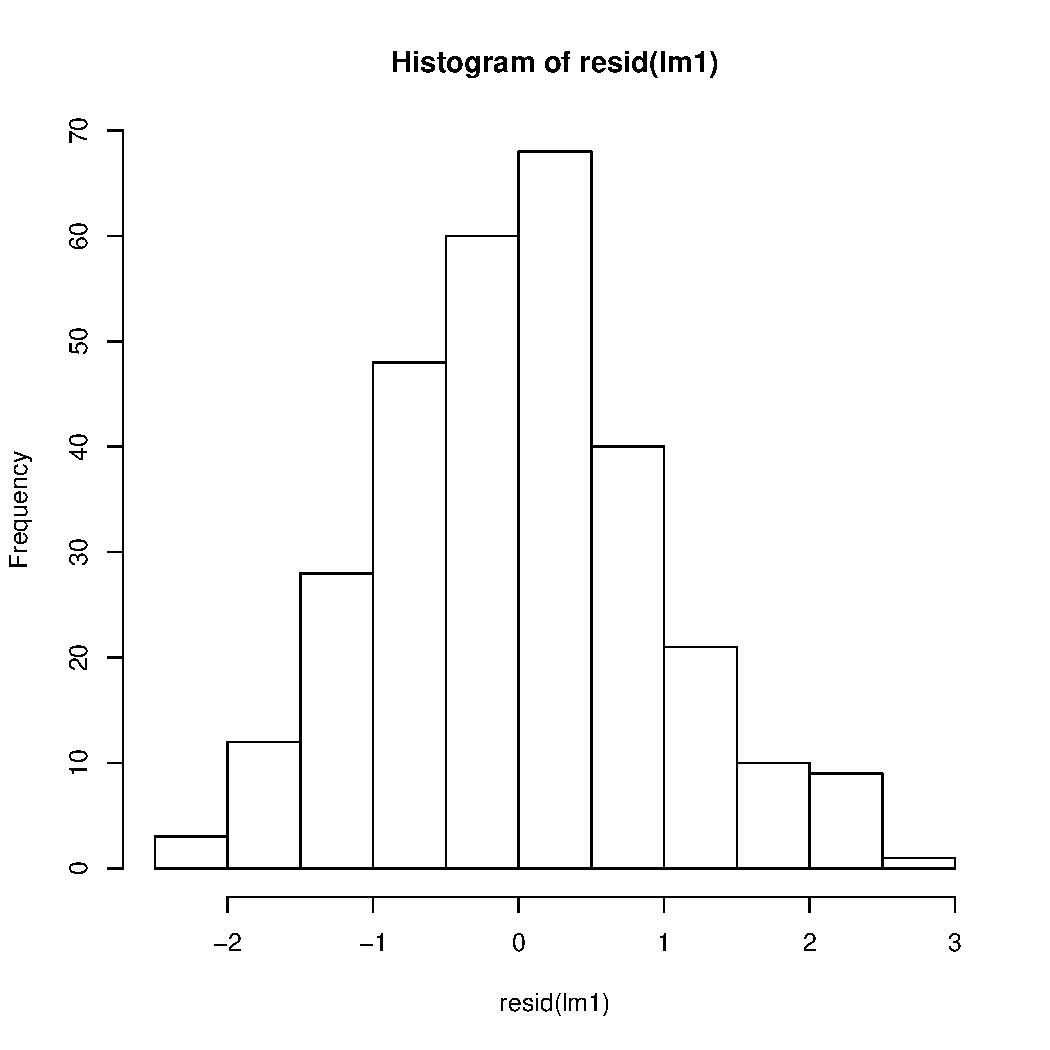
\includegraphics[width=\maxwidth]{figure/unnamed-chunk-3-1} 
\begin{kframe}\begin{alltt}
\hlkwd{hist}\hlstd{(}\hlkwd{resid}\hlstd{(lm2))}
\end{alltt}
\end{kframe}
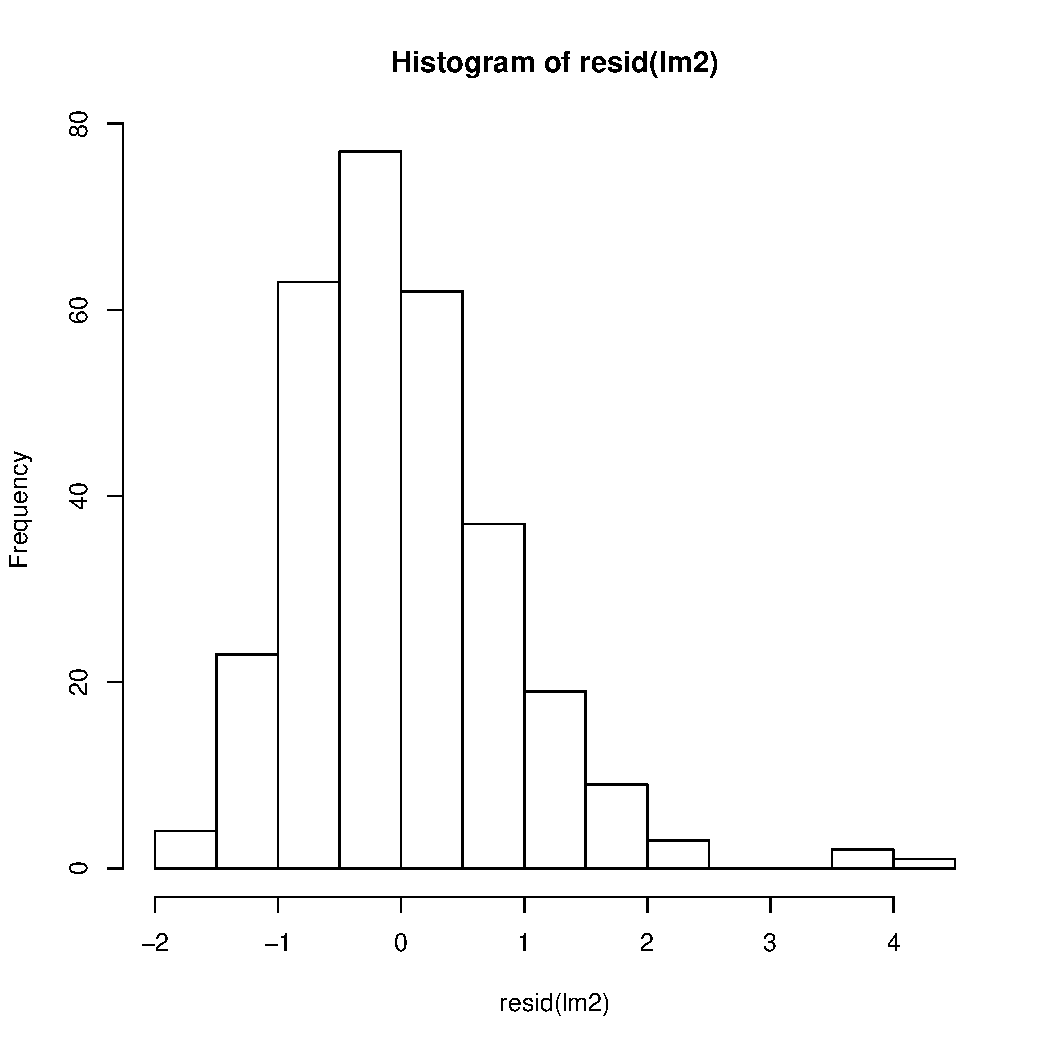
\includegraphics[width=\maxwidth]{figure/unnamed-chunk-3-2} 
\begin{kframe}\begin{alltt}
\hlkwd{hist}\hlstd{(}\hlkwd{resid}\hlstd{(lm3))}
\end{alltt}
\end{kframe}
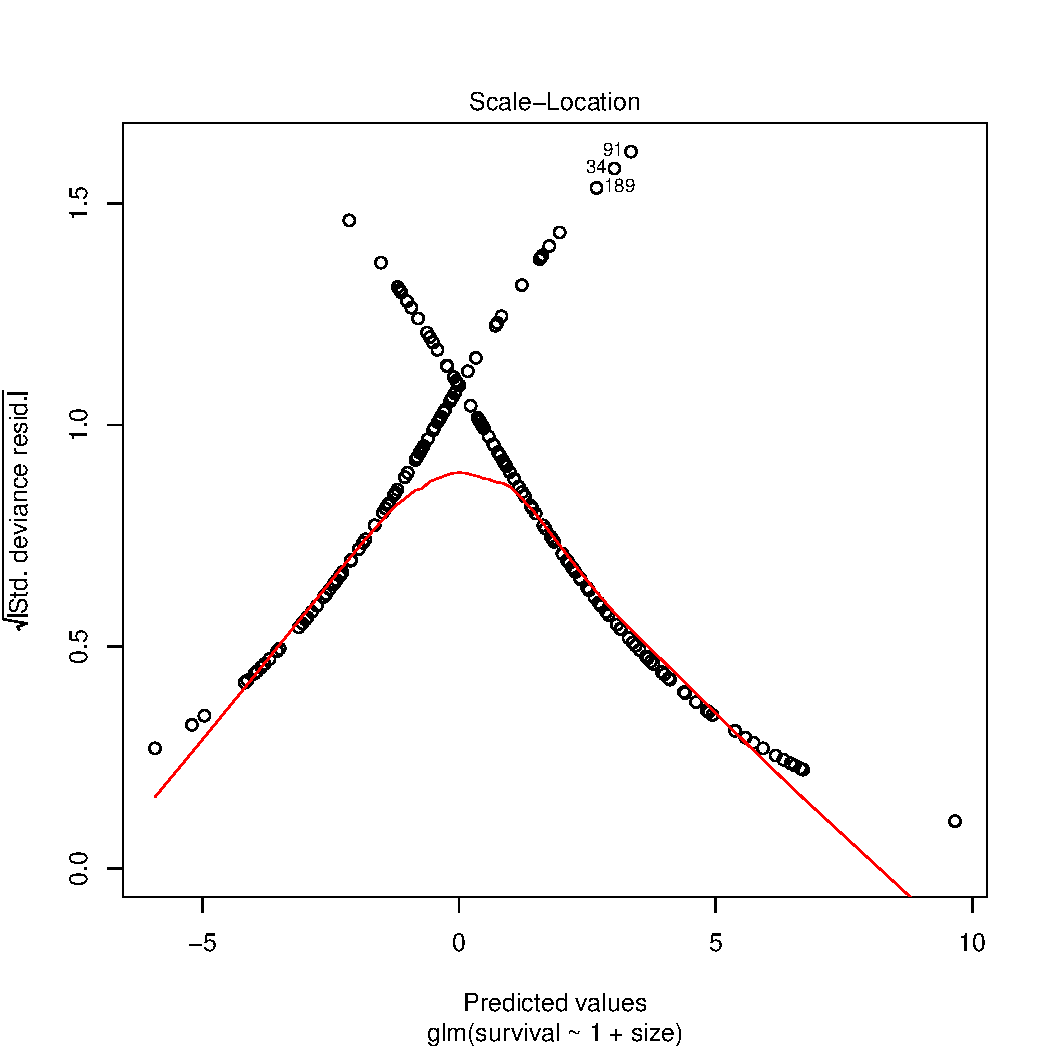
\includegraphics[width=\maxwidth]{figure/unnamed-chunk-3-3} 

\end{knitrout}

The model with response1 is okay: the residual are normally distributed. The two others are not right. You could log-transform response2 because it is continuous and does not include zeroes. For response3 it would be better to fit a Poisson generalized linear model because the data are integer only (and contain zeroes).
\end{Answer}


\begin{Exercise}[difficulty=1, title={What is missing?}]


Load the dataset \texttt{boldness.csv}. We want to know how boldness relates to size and we fit a simple linear model of boldness as a function of size. Check the assumptions of such a model. What is wrong, how to fix it?
\end{Exercise}
\begin{Answer}
\begin{knitrout}
\definecolor{shadecolor}{rgb}{0.969, 0.969, 0.969}\color{fgcolor}\begin{kframe}
\begin{alltt}
\hlstd{dat} \hlkwb{<-} \hlkwd{read.csv}\hlstd{(}\hlstr{"boldness.csv"}\hlstd{)}
\hlstd{lm0} \hlkwb{<-} \hlkwd{lm}\hlstd{(boldness}\hlopt{~}\hlstd{size,} \hlkwc{data} \hlstd{= dat)}
\hlkwd{plot}\hlstd{(lm0)}
\end{alltt}
\end{kframe}
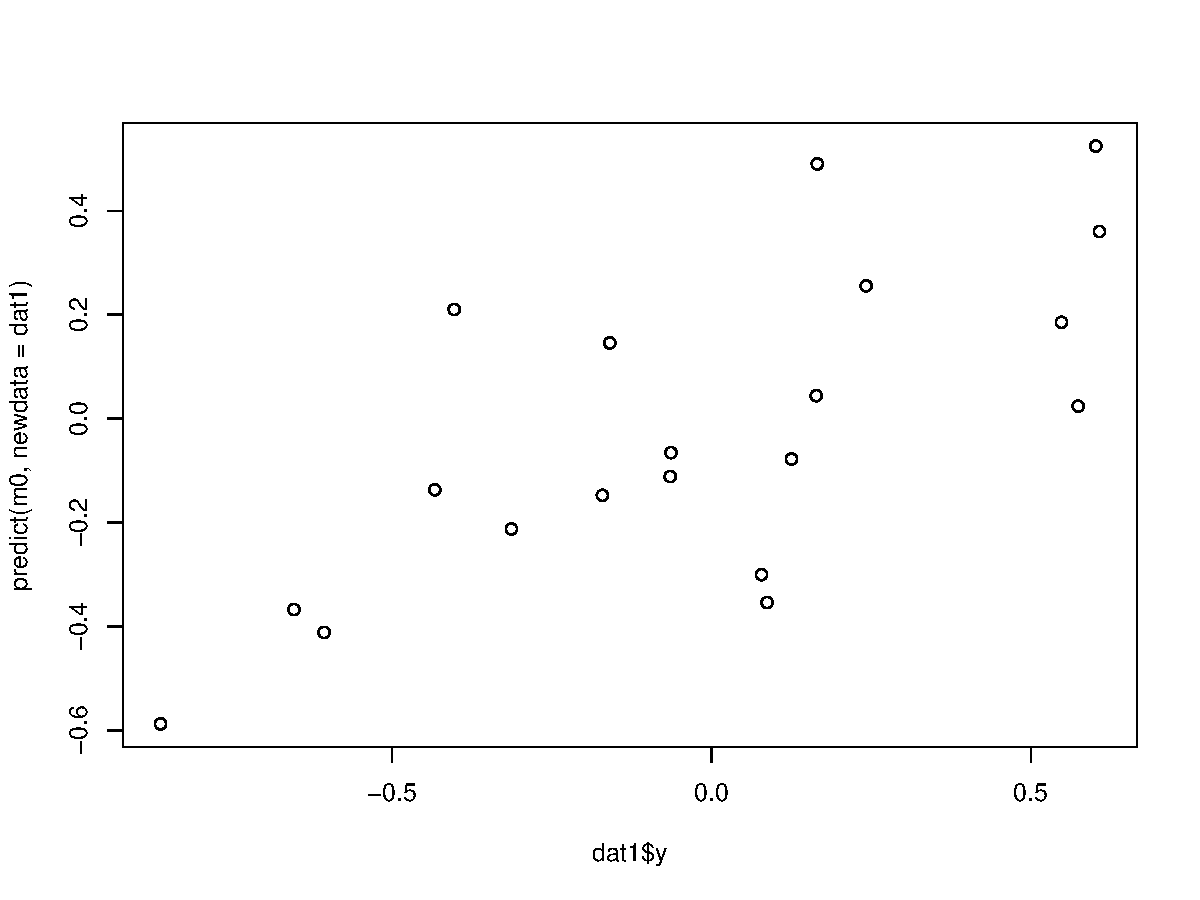
\includegraphics[width=\maxwidth]{figure/unnamed-chunk-5-1} 

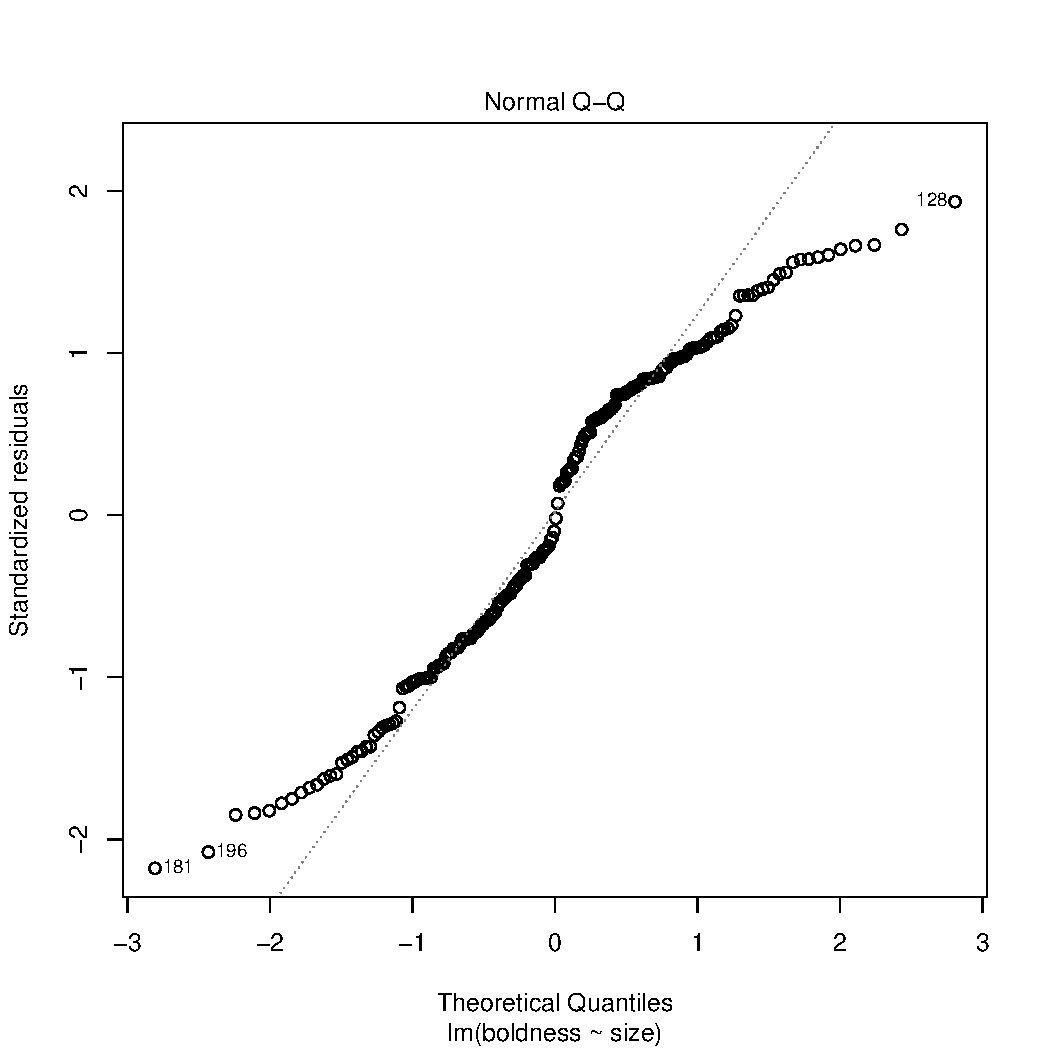
\includegraphics[width=\maxwidth]{figure/unnamed-chunk-5-2} 

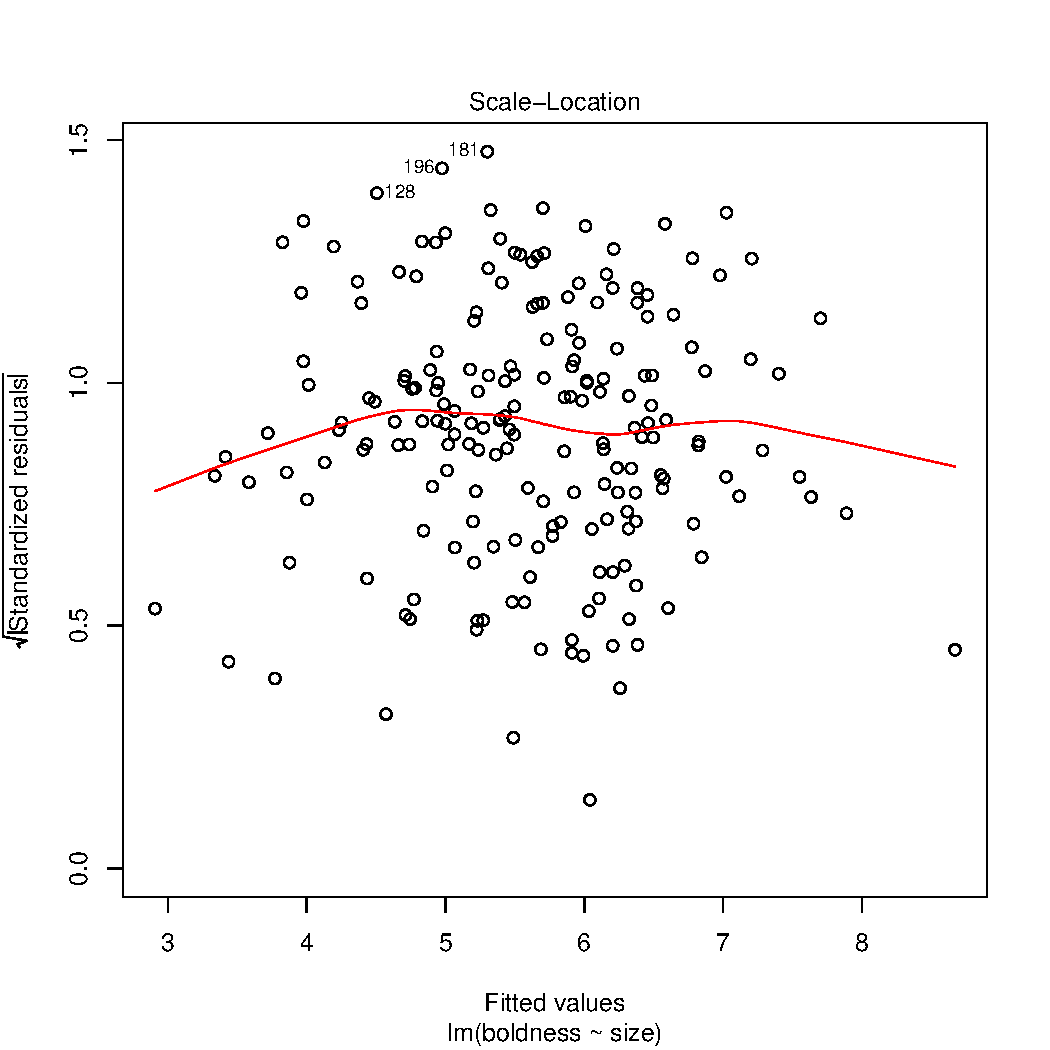
\includegraphics[width=\maxwidth]{figure/unnamed-chunk-5-3} 

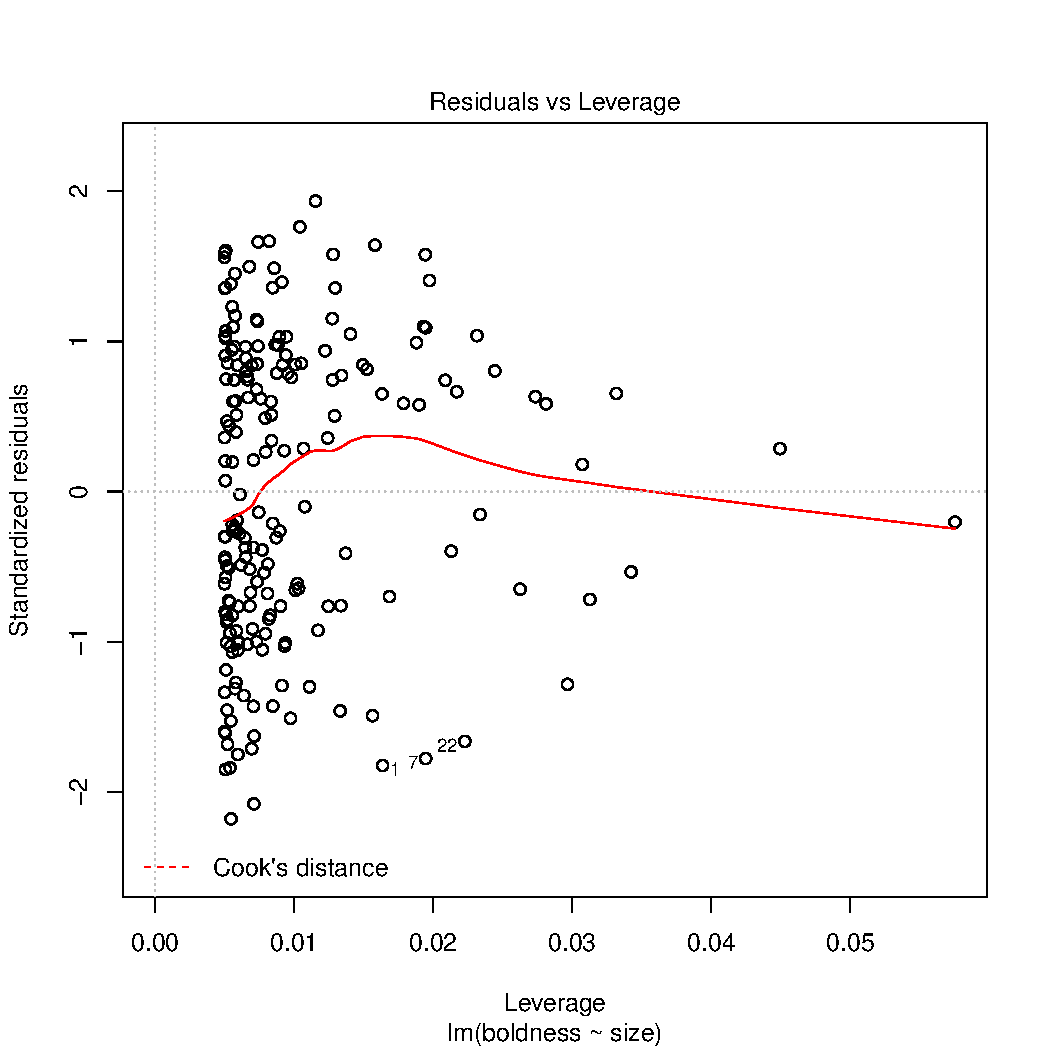
\includegraphics[width=\maxwidth]{figure/unnamed-chunk-5-4} 

\end{knitrout}
The residuals are not normally distributed; they look like a mixture of two normal distribution, that is, they are bimodal.
\begin{knitrout}
\definecolor{shadecolor}{rgb}{0.969, 0.969, 0.969}\color{fgcolor}\begin{kframe}
\begin{alltt}
\hlkwd{hist}\hlstd{(}\hlkwd{resid}\hlstd{(lm0))}
\end{alltt}
\end{kframe}
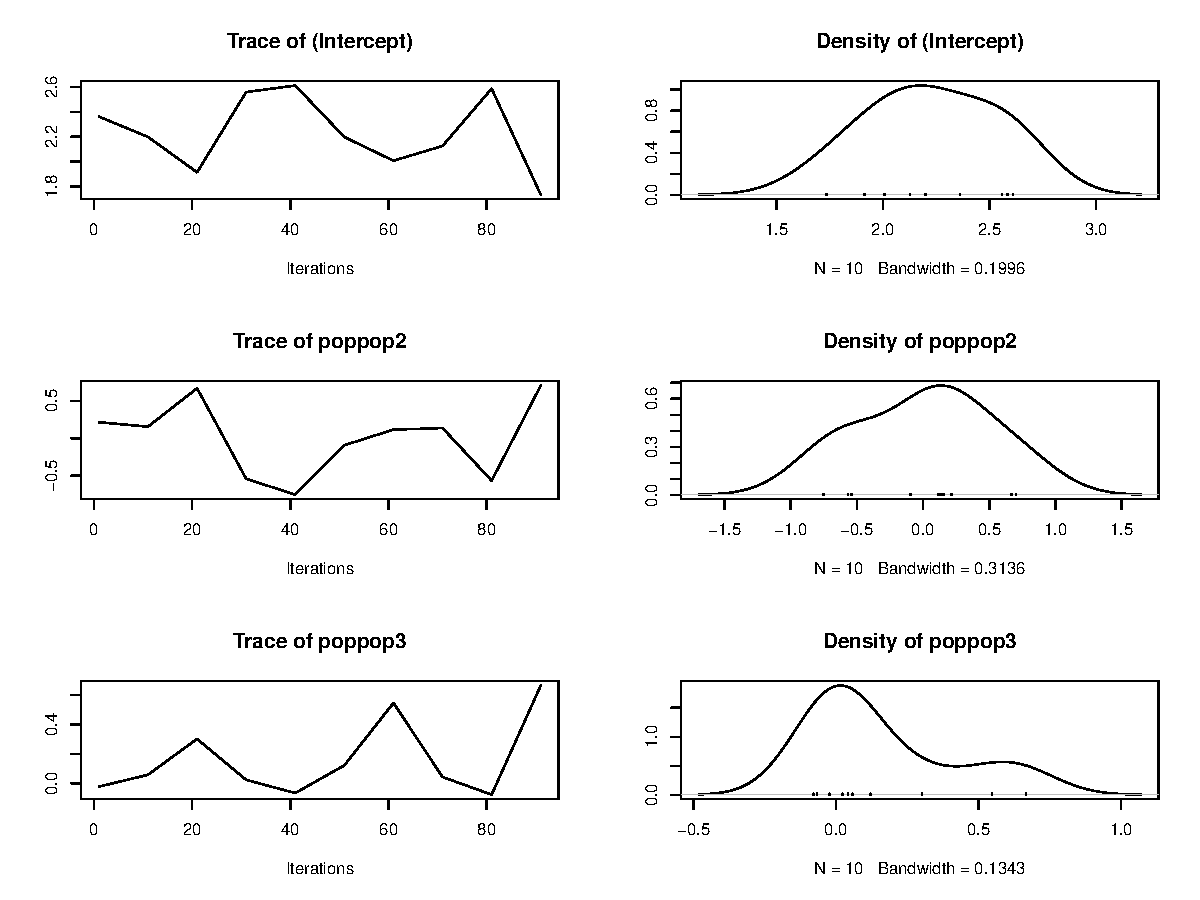
\includegraphics[width=\maxwidth]{figure/unnamed-chunk-6-1} 

\end{knitrout}

There are other covariates in the data set. One of them may be a crucial factor explaining boldness. If you look at plots of the data:
\begin{knitrout}
\definecolor{shadecolor}{rgb}{0.969, 0.969, 0.969}\color{fgcolor}\begin{kframe}
\begin{alltt}
\hlkwd{plot}\hlstd{(dat)}
\end{alltt}
\end{kframe}
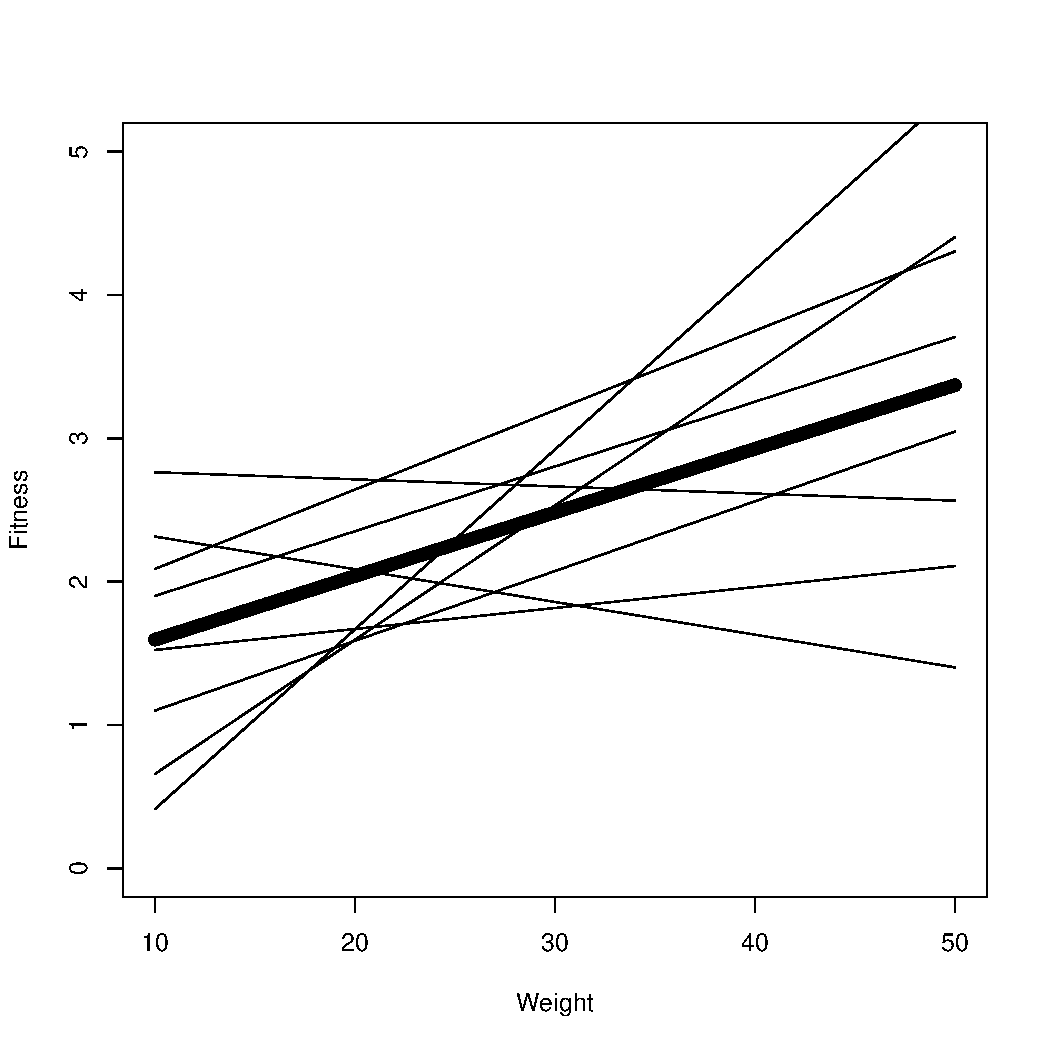
\includegraphics[width=\maxwidth]{figure/unnamed-chunk-7-1} 

\end{knitrout}
you may notice that sex is important.
So, include sex in your model:
\begin{knitrout}
\definecolor{shadecolor}{rgb}{0.969, 0.969, 0.969}\color{fgcolor}\begin{kframe}
\begin{alltt}
\hlstd{lm1} \hlkwb{<-} \hlkwd{lm}\hlstd{(boldness}\hlopt{~}\hlstd{size}\hlopt{+}\hlstd{sex,} \hlkwc{data} \hlstd{= dat)}
\hlkwd{plot}\hlstd{(lm1)}
\end{alltt}
\end{kframe}
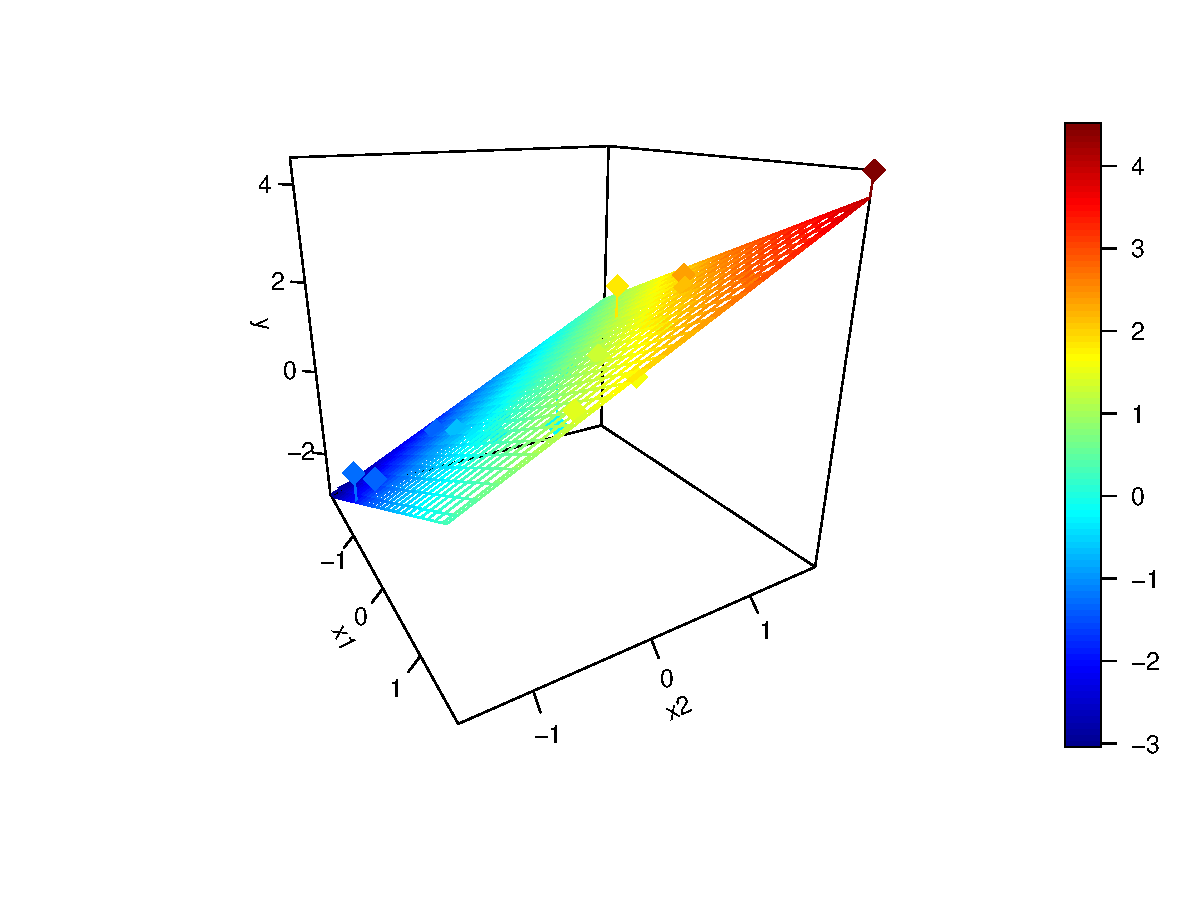
\includegraphics[width=\maxwidth]{figure/unnamed-chunk-8-1} 

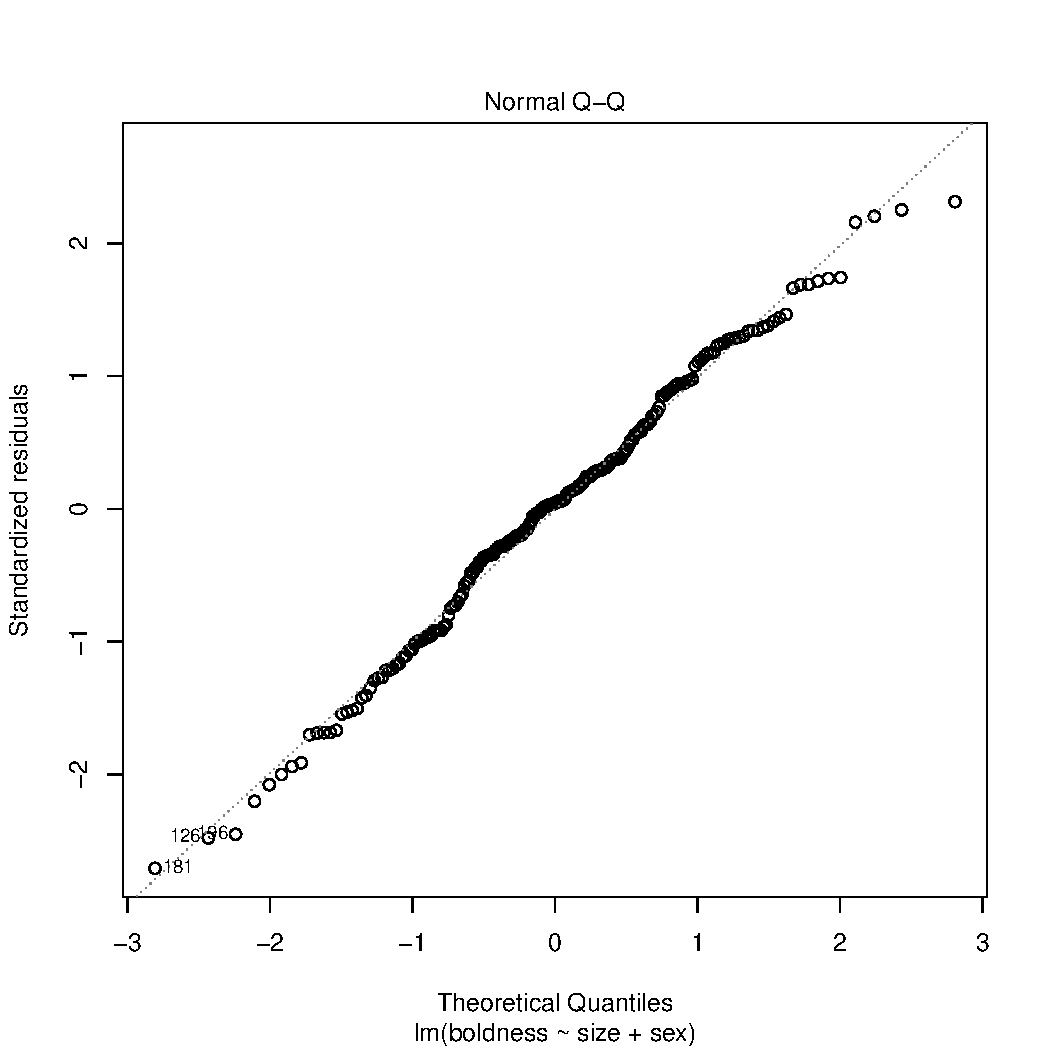
\includegraphics[width=\maxwidth]{figure/unnamed-chunk-8-2} 

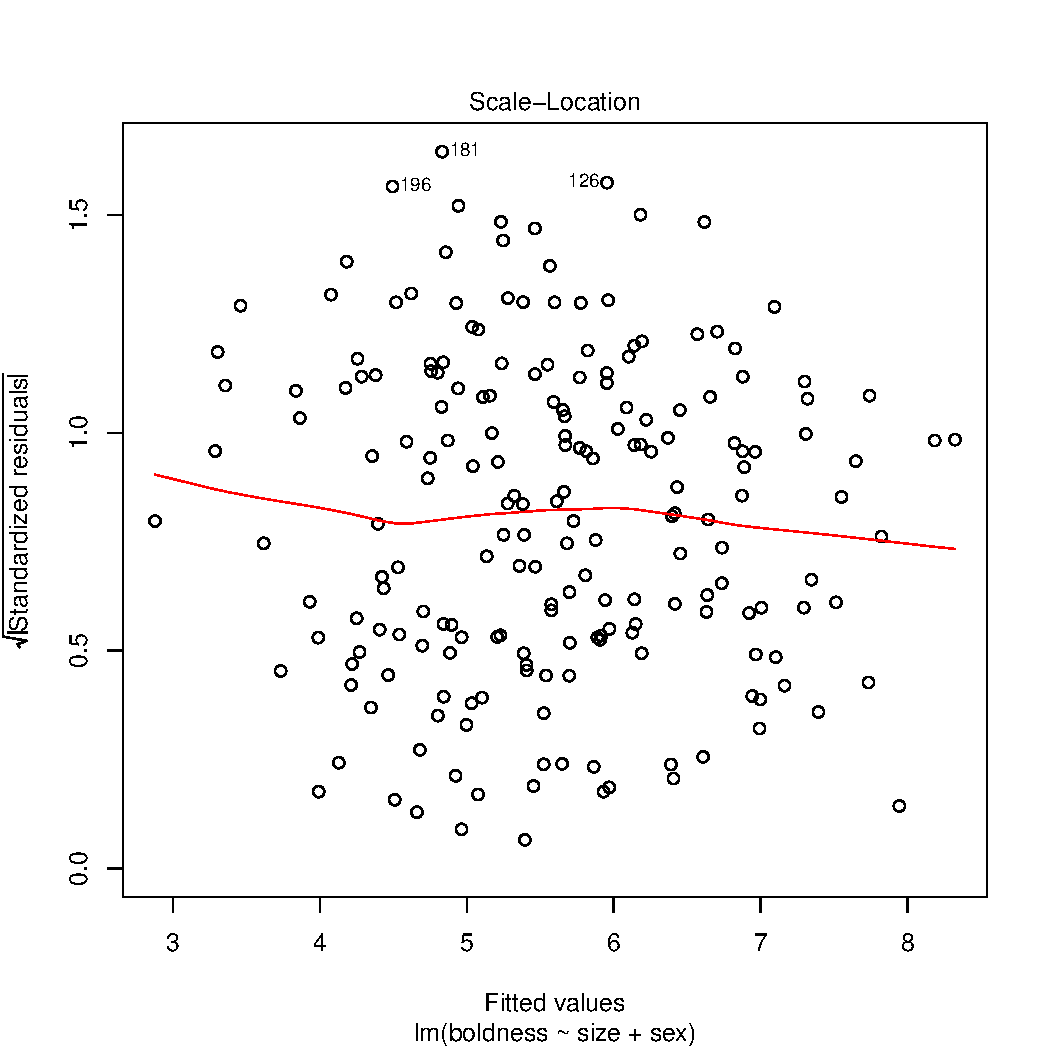
\includegraphics[width=\maxwidth]{figure/unnamed-chunk-8-3} 

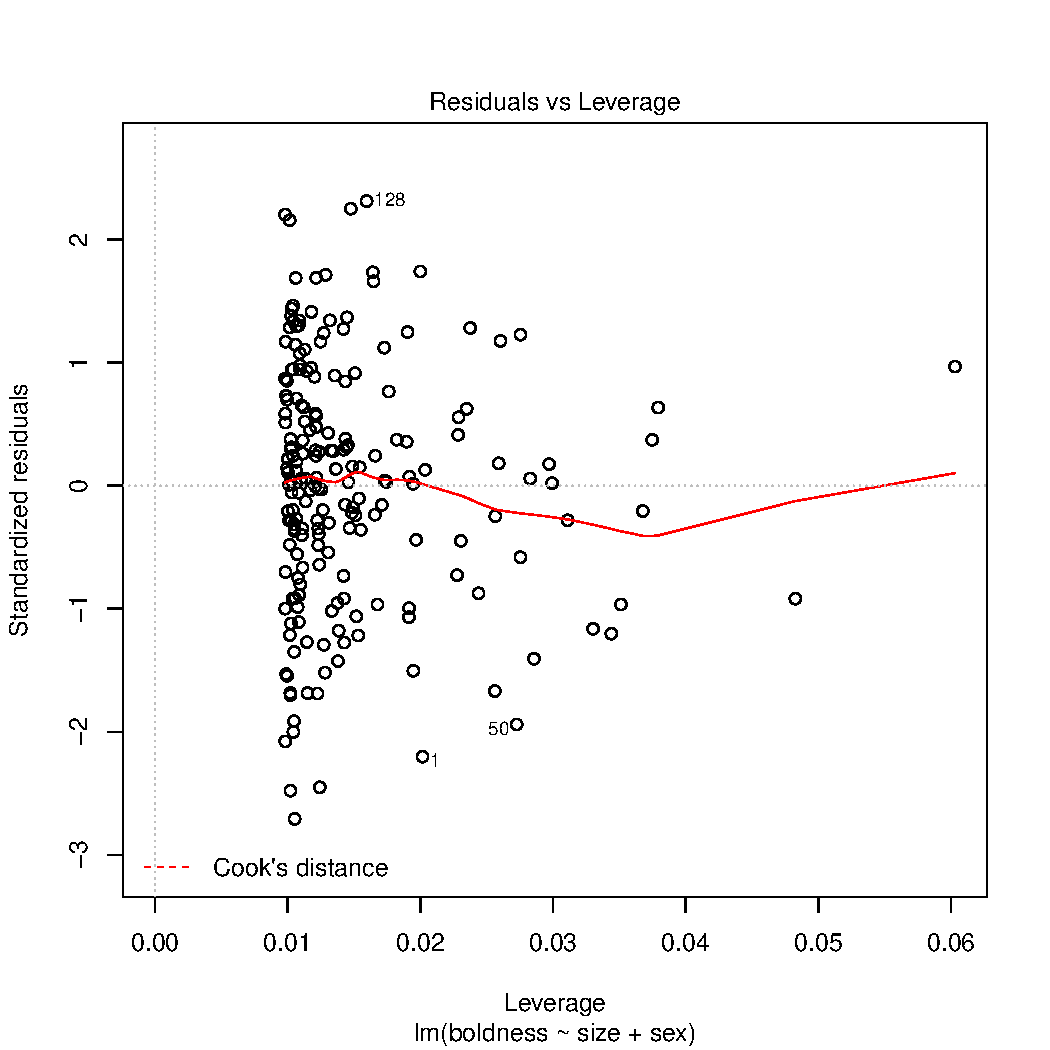
\includegraphics[width=\maxwidth]{figure/unnamed-chunk-8-4} 

\end{knitrout}
Very nice!
\end{Answer}

\section{Non-independence}

\begin{Exercise}[difficulty=1, title={Simpson's paradox}]
Load the dataset \texttt{thorndata.txt}. According to simple linear models, does thorns have an effect on herbivory? Is the effect consistent across sites (fit models on subsets)? 
\end{Exercise}
\begin{Answer}
\begin{knitrout}
\definecolor{shadecolor}{rgb}{0.969, 0.969, 0.969}\color{fgcolor}\begin{kframe}
\begin{alltt}
\hlstd{thorns} \hlkwb{<-} \hlkwd{read.table}\hlstd{(}\hlstr{"thorndata.txt"}\hlstd{,} \hlkwc{header} \hlstd{=} \hlnum{TRUE}\hlstd{)}
\hlkwd{summary}\hlstd{(lm0} \hlkwb{<-} \hlkwd{lm}\hlstd{(}\hlkwc{data} \hlstd{= thorns,} \hlkwc{formula} \hlstd{= herbivory} \hlopt{~} \hlnum{1}\hlopt{+}\hlstd{thorndensity ))}
\end{alltt}
\begin{verbatim}
## 
## Call:
## lm(formula = herbivory ~ 1 + thorndensity, data = thorns)
## 
## Residuals:
##     Min      1Q  Median      3Q     Max 
## -2.1162 -0.5183  0.0821  0.5435  1.5193 
## 
## Coefficients:
##              Estimate Std. Error t value Pr(>|t|)    
## (Intercept)    3.2564     0.2854   11.41  < 2e-16 ***
## thorndensity   0.2524     0.0717    3.52  0.00066 ***
## ---
## Signif. codes:  0 '***' 0.001 '**' 0.01 '*' 0.05 '.' 0.1 ' ' 1
## 
## Residual standard error: 0.725 on 98 degrees of freedom
## Multiple R-squared:  0.112,	Adjusted R-squared:  0.103 
## F-statistic: 12.4 on 1 and 98 DF,  p-value: 0.000657
\end{verbatim}
\begin{alltt}
\hlkwd{plot}\hlstd{(lm0)}
\end{alltt}
\end{kframe}
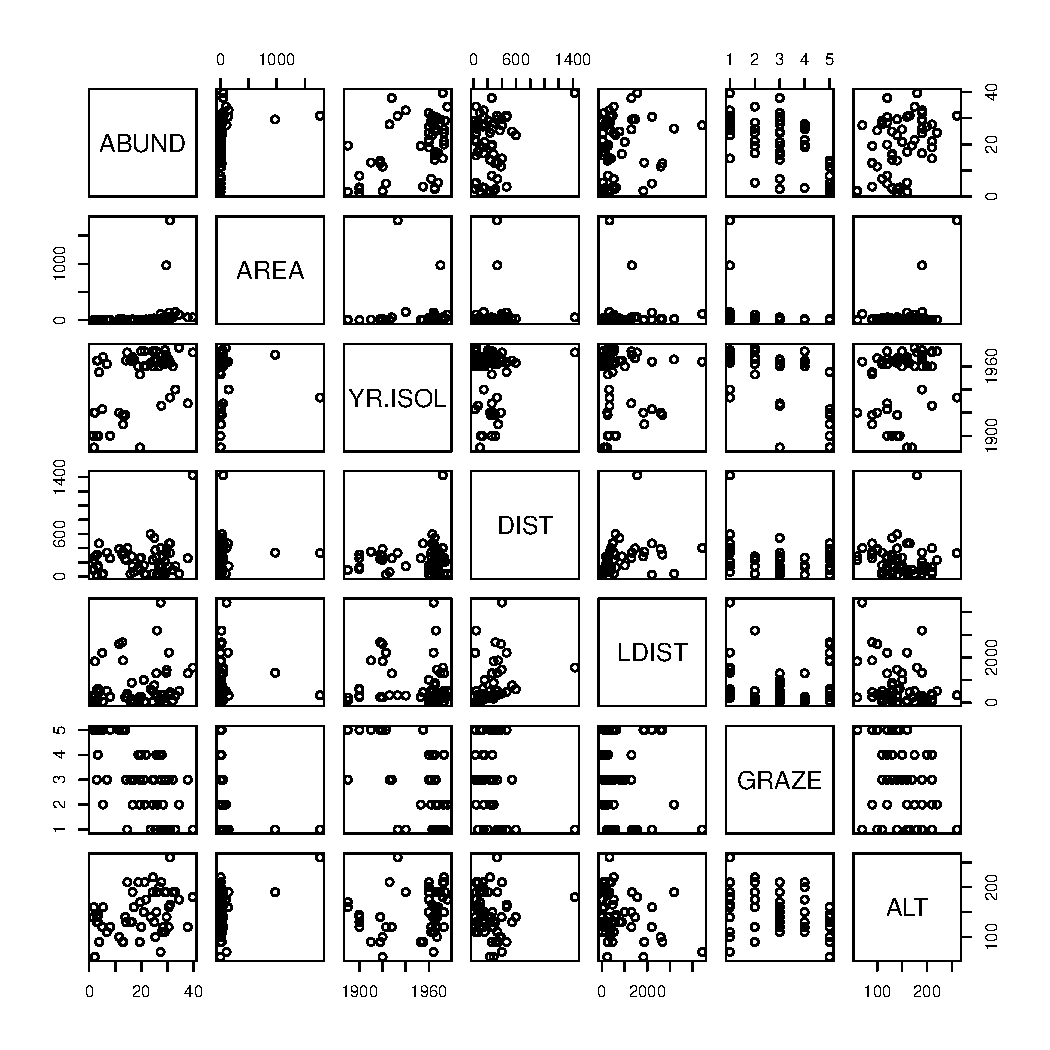
\includegraphics[width=\maxwidth]{figure/unnamed-chunk-9-1} 

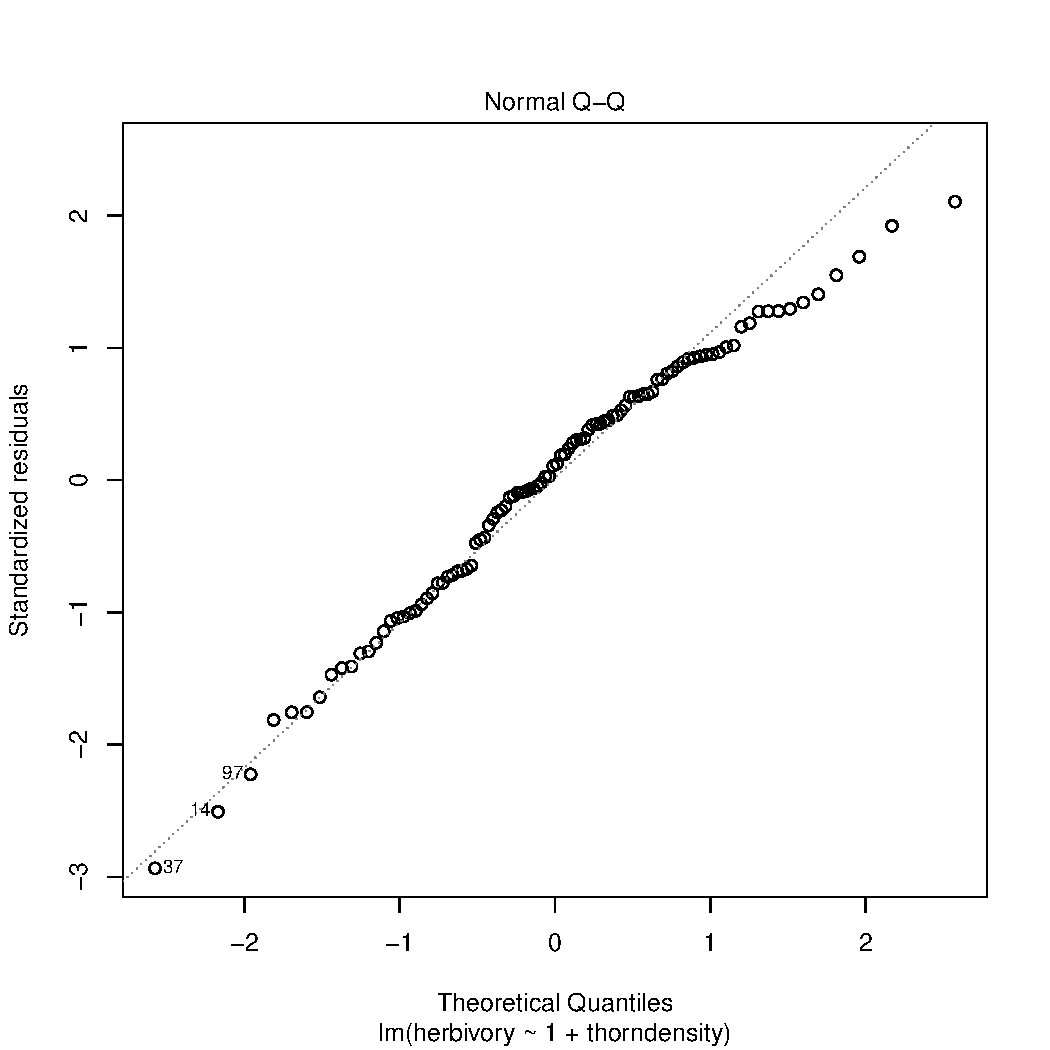
\includegraphics[width=\maxwidth]{figure/unnamed-chunk-9-2} 

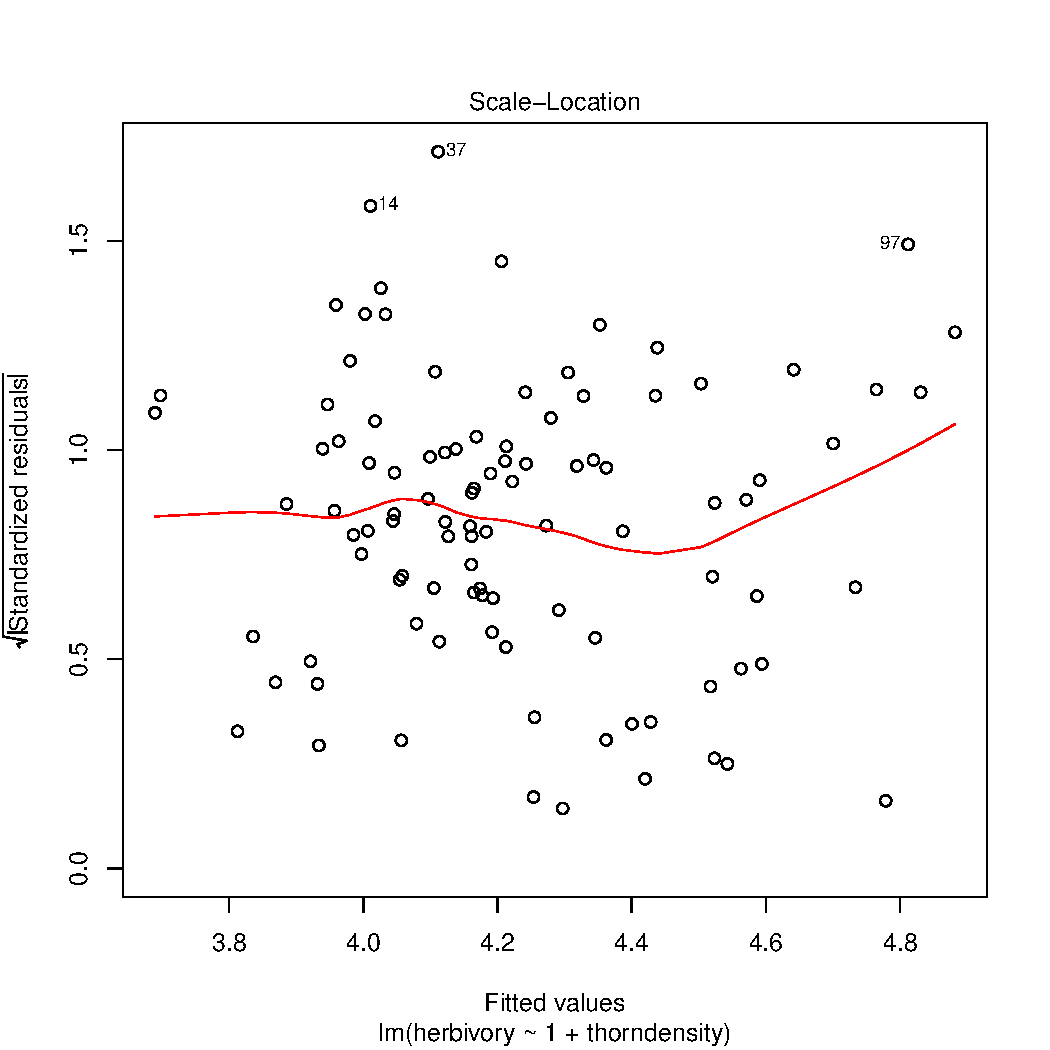
\includegraphics[width=\maxwidth]{figure/unnamed-chunk-9-3} 

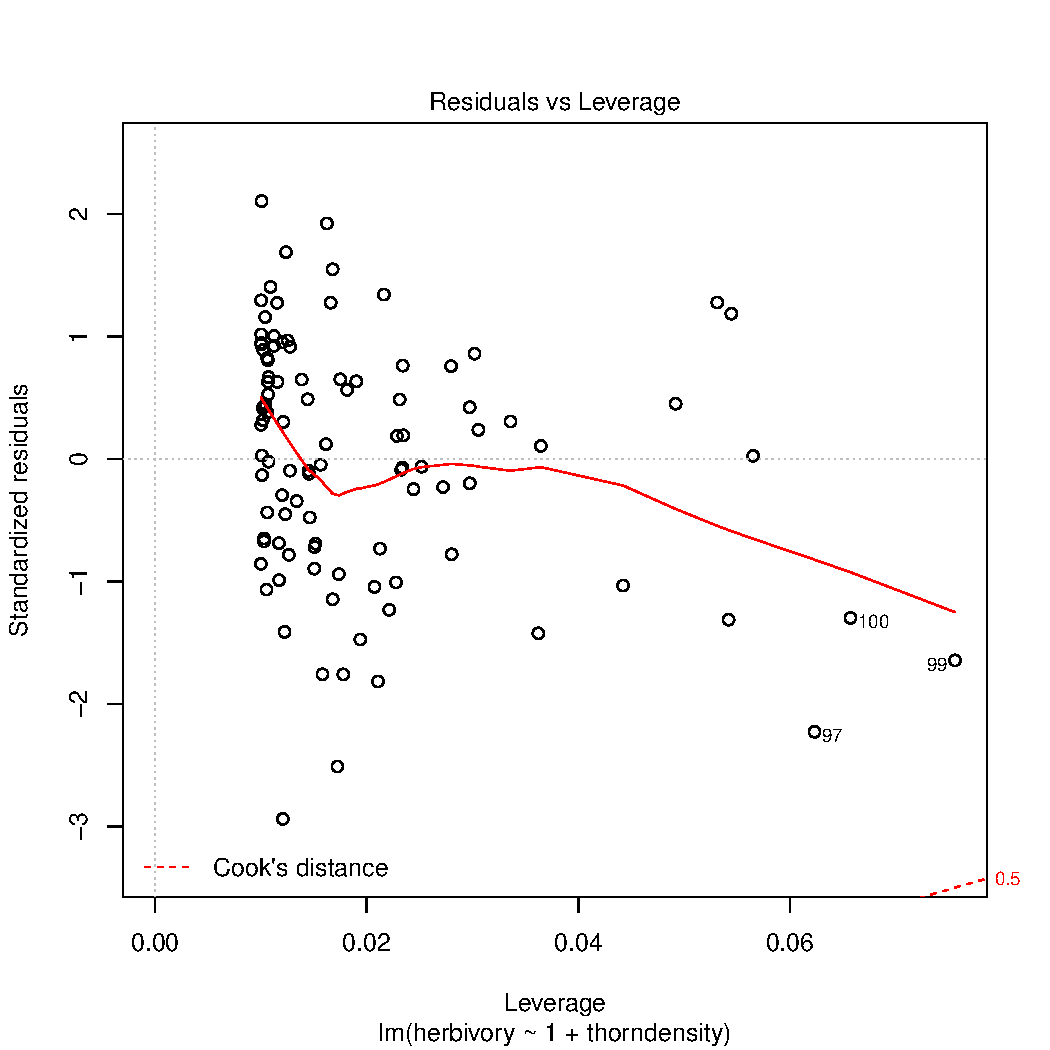
\includegraphics[width=\maxwidth]{figure/unnamed-chunk-9-4} 
\begin{kframe}\begin{alltt}
\hlkwd{summary}\hlstd{(lm1} \hlkwb{<-} \hlkwd{lm}\hlstd{(}\hlkwc{data} \hlstd{= thorns ,} \hlkwc{formula} \hlstd{= herbivory} \hlopt{~} \hlnum{1}\hlopt{+}\hlstd{thorndensity}\hlopt{+} \hlstd{site ))}
\end{alltt}
\begin{verbatim}
## 
## Call:
## lm(formula = herbivory ~ 1 + thorndensity + site, data = thorns)
## 
## Residuals:
##     Min      1Q  Median      3Q     Max 
## -1.7123 -0.2724  0.0476  0.2456  1.3492 
## 
## Coefficients:
##              Estimate Std. Error t value Pr(>|t|)    
## (Intercept)     5.239      0.261   20.11  < 2e-16 ***
## thorndensity   -1.043      0.126   -8.29  6.5e-13 ***
## site            1.002      0.090   11.13  < 2e-16 ***
## ---
## Signif. codes:  0 '***' 0.001 '**' 0.01 '*' 0.05 '.' 0.1 ' ' 1
## 
## Residual standard error: 0.483 on 97 degrees of freedom
## Multiple R-squared:  0.61,	Adjusted R-squared:  0.602 
## F-statistic: 75.8 on 2 and 97 DF,  p-value: <2e-16
\end{verbatim}
\begin{alltt}
\hlcom{#or using a mixed model}
\hlkwd{library}\hlstd{(lme4)}
\hlkwd{summary}\hlstd{(lmm2} \hlkwb{<-} \hlkwd{lmer}\hlstd{(}\hlkwc{data} \hlstd{= thorns ,} \hlkwc{formula} \hlstd{= herbivory} \hlopt{~} \hlnum{1}\hlopt{+}\hlstd{thorndensity}\hlopt{+} \hlstd{(}\hlnum{1}\hlopt{|}\hlstd{site )))}
\end{alltt}
\begin{verbatim}
## Linear mixed model fit by REML ['lmerMod']
## Formula: herbivory ~ 1 + thorndensity + (1 | site)
##    Data: thorns
## 
## REML criterion at convergence: 165.3
## 
## Scaled residuals: 
##    Min     1Q Median     3Q    Max 
## -3.488 -0.606  0.109  0.523  2.873 
## 
## Random effects:
##  Groups   Name        Variance Std.Dev.
##  site     (Intercept) 2.129    1.459   
##  Residual             0.238    0.488   
## Number of obs: 100, groups:  site, 5
## 
## Fixed effects:
##              Estimate Std. Error t value
## (Intercept)     7.765      0.844    9.20
## thorndensity   -0.919      0.139   -6.63
## 
## Correlation of Fixed Effects:
##             (Intr)
## thorndensty -0.632
\end{verbatim}
\end{kframe}
\end{knitrout}

\begin{knitrout}
\definecolor{shadecolor}{rgb}{0.969, 0.969, 0.969}\color{fgcolor}\begin{kframe}
\begin{alltt}
\hlkwd{library}\hlstd{(ggplot2)}
\end{alltt}


{\ttfamily\noindent\itshape\color{messagecolor}{\#\# Registered S3 methods overwritten by 'ggplot2':\\\#\#\ \  method\ \ \ \ \ \ \ \  from \\\#\#\ \  [.quosures\ \ \ \  rlang\\\#\#\ \  c.quosures\ \ \ \  rlang\\\#\#\ \  print.quosures rlang}}\begin{alltt}
\hlkwd{ggplot}\hlstd{(}\hlkwc{data}\hlstd{=thorns,} \hlkwd{aes}\hlstd{(}\hlkwc{y}\hlstd{=herbivory,} \hlkwc{x}\hlstd{=thorndensity,} \hlkwc{color}\hlstd{=}\hlkwd{as.factor}\hlstd{(site)))} \hlopt{+} \hlkwd{geom_point}\hlstd{()}
\end{alltt}
\end{kframe}
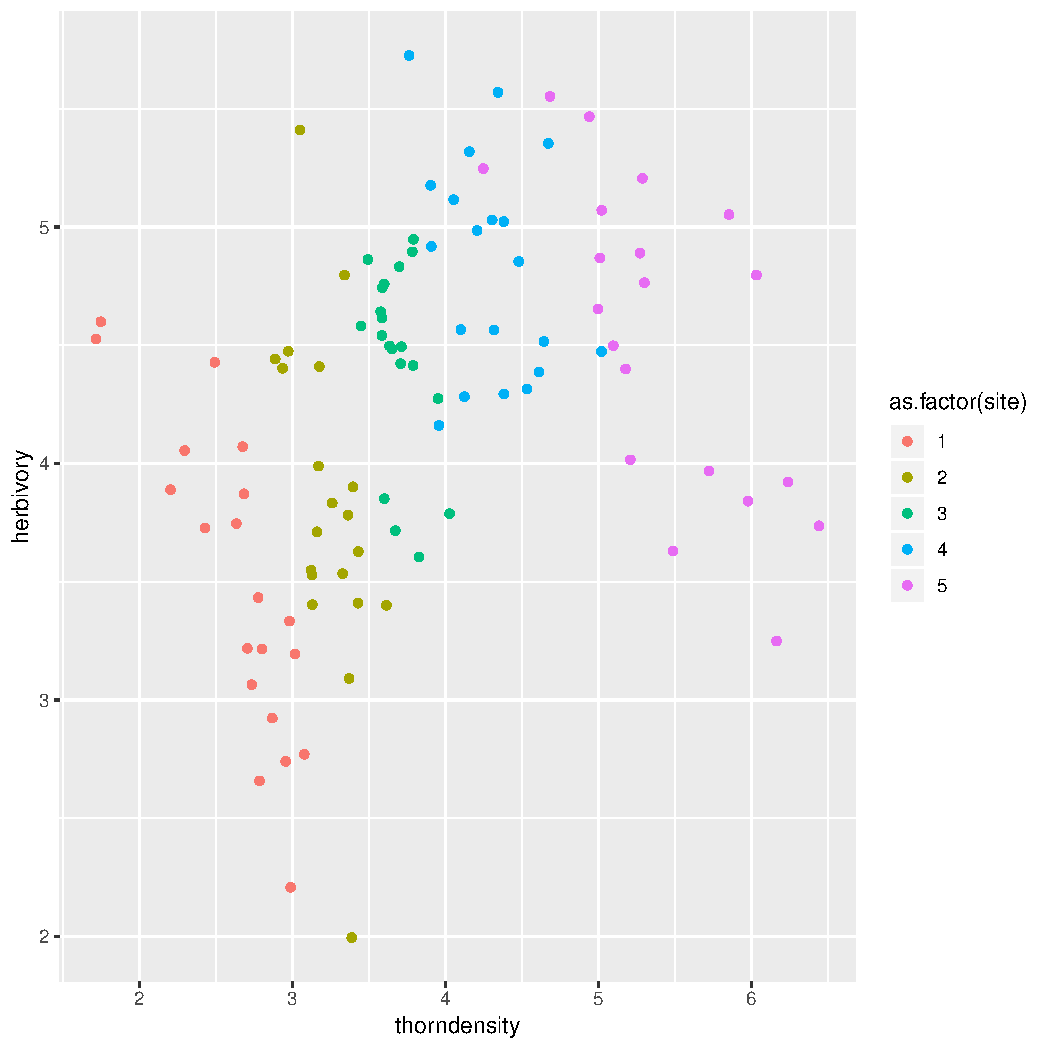
\includegraphics[width=\maxwidth]{figure/unnamed-chunk-10-1} 

\end{knitrout}
\end{Answer}


\begin{Exercise}[difficulty=2, title={Genetic isolation distance or adaptation?}]


Load the dataset \texttt{genotype.csv}. Let's imagine that in a tree species we have measured allele frequencies at a gene that we suspect is related to thermal adaptation. Fit a simple linear model of AllFreq as a function of temperature. Check model assumptions. Are you confident this gene controls local adaptation to temperature?
\end{Exercise}
\begin{Answer}
\begin{knitrout}
\definecolor{shadecolor}{rgb}{0.969, 0.969, 0.969}\color{fgcolor}\begin{kframe}
\begin{alltt}
\hlstd{genot} \hlkwb{<-} \hlkwd{read.csv}\hlstd{(}\hlstr{"genotype.csv"}\hlstd{)}
\hlstd{lm0} \hlkwb{<-} \hlkwd{lm}\hlstd{(AllFreq} \hlopt{~} \hlnum{1} \hlopt{+} \hlstd{temperature,} \hlkwc{data}\hlstd{=genot)}
\hlkwd{summary}\hlstd{(lm0)}
\end{alltt}
\begin{verbatim}
## 
## Call:
## lm(formula = AllFreq ~ 1 + temperature, data = genot)
## 
## Residuals:
##      Min       1Q   Median       3Q      Max 
## -0.24625 -0.10051  0.00363  0.11672  0.19836 
## 
## Coefficients:
##             Estimate Std. Error t value Pr(>|t|)    
## (Intercept)  -4.2076     0.7638   -5.51  1.4e-06 ***
## temperature   0.4542     0.0736    6.17  1.4e-07 ***
## ---
## Signif. codes:  0 '***' 0.001 '**' 0.01 '*' 0.05 '.' 0.1 ' ' 1
## 
## Residual standard error: 0.124 on 48 degrees of freedom
## Multiple R-squared:  0.442,	Adjusted R-squared:  0.43 
## F-statistic:   38 on 1 and 48 DF,  p-value: 1.4e-07
\end{verbatim}
\begin{alltt}
\hlkwd{plot}\hlstd{(lm0)}
\end{alltt}
\end{kframe}
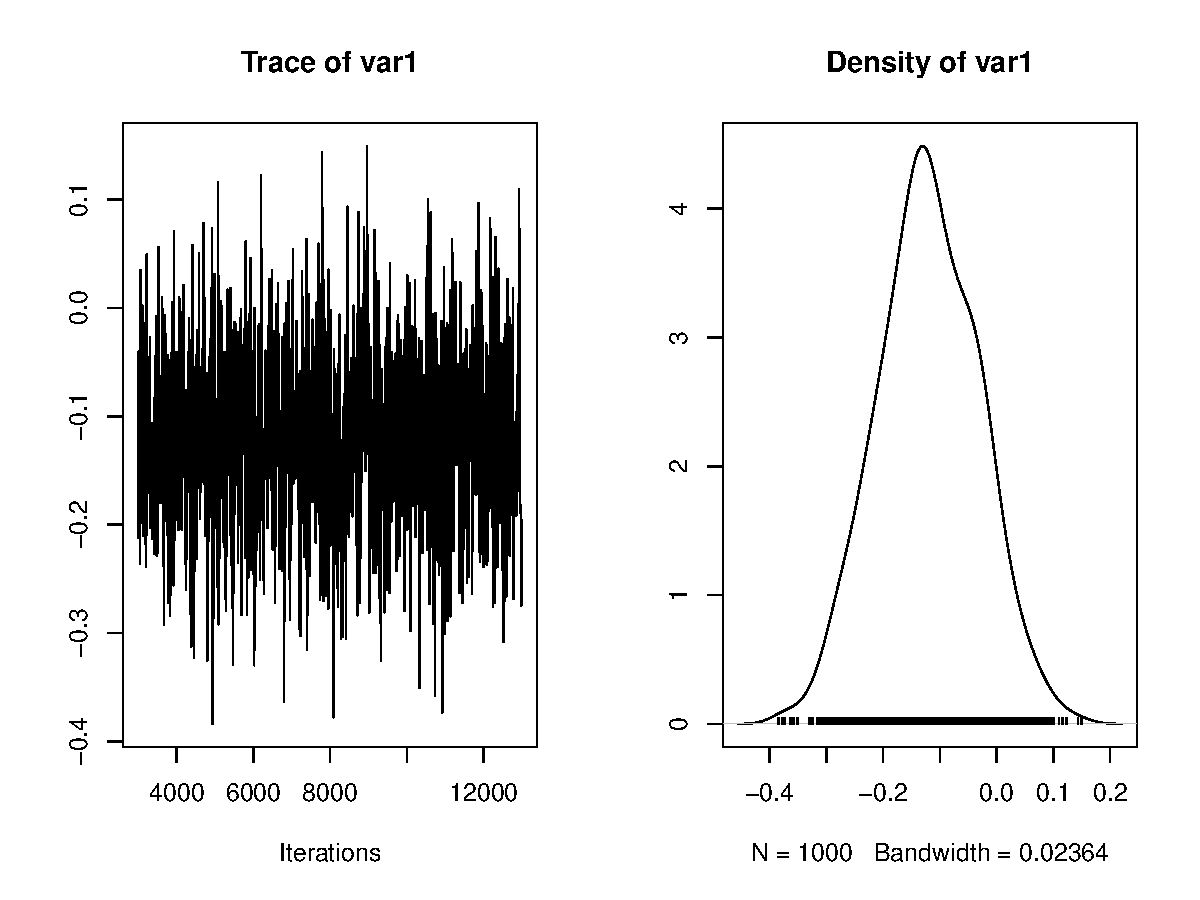
\includegraphics[width=\maxwidth]{figure/unnamed-chunk-12-1} 

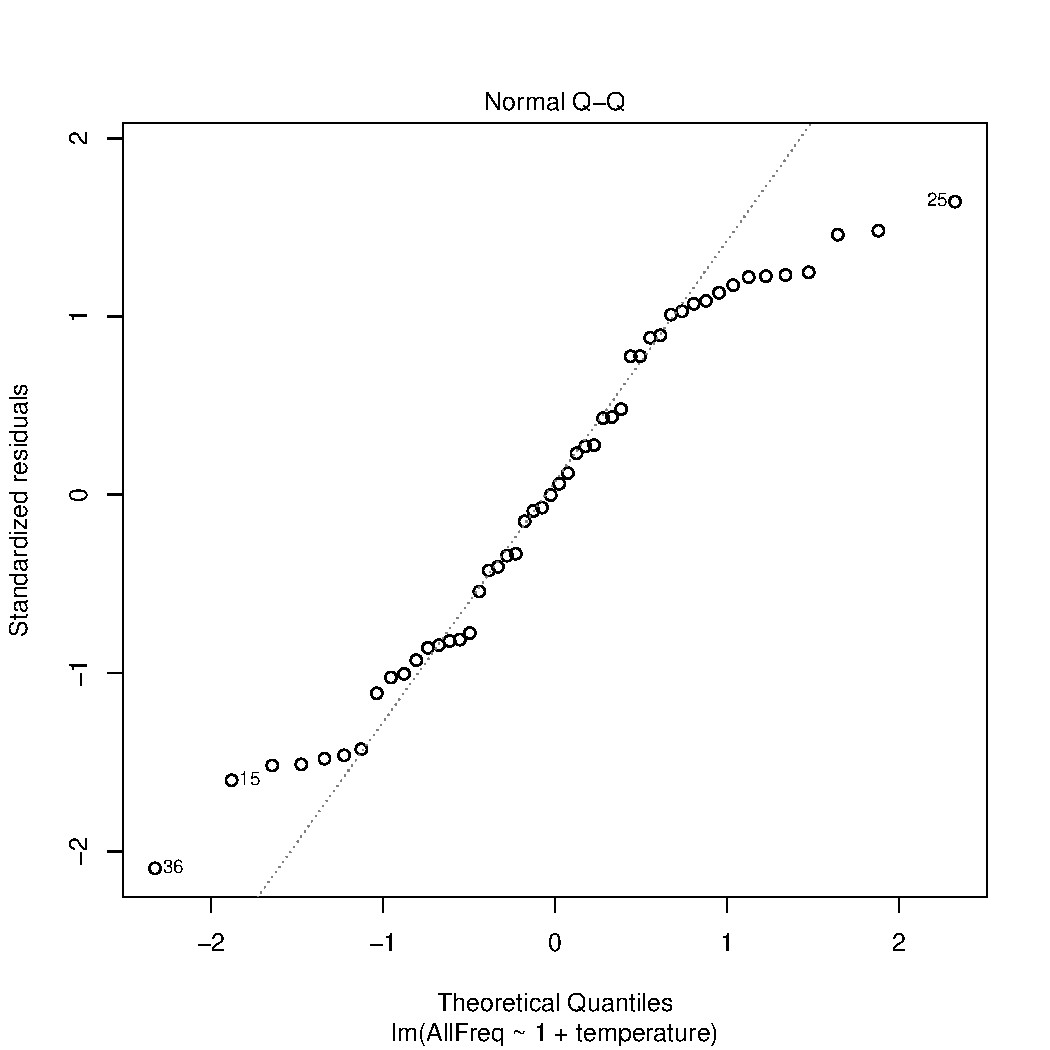
\includegraphics[width=\maxwidth]{figure/unnamed-chunk-12-2} 

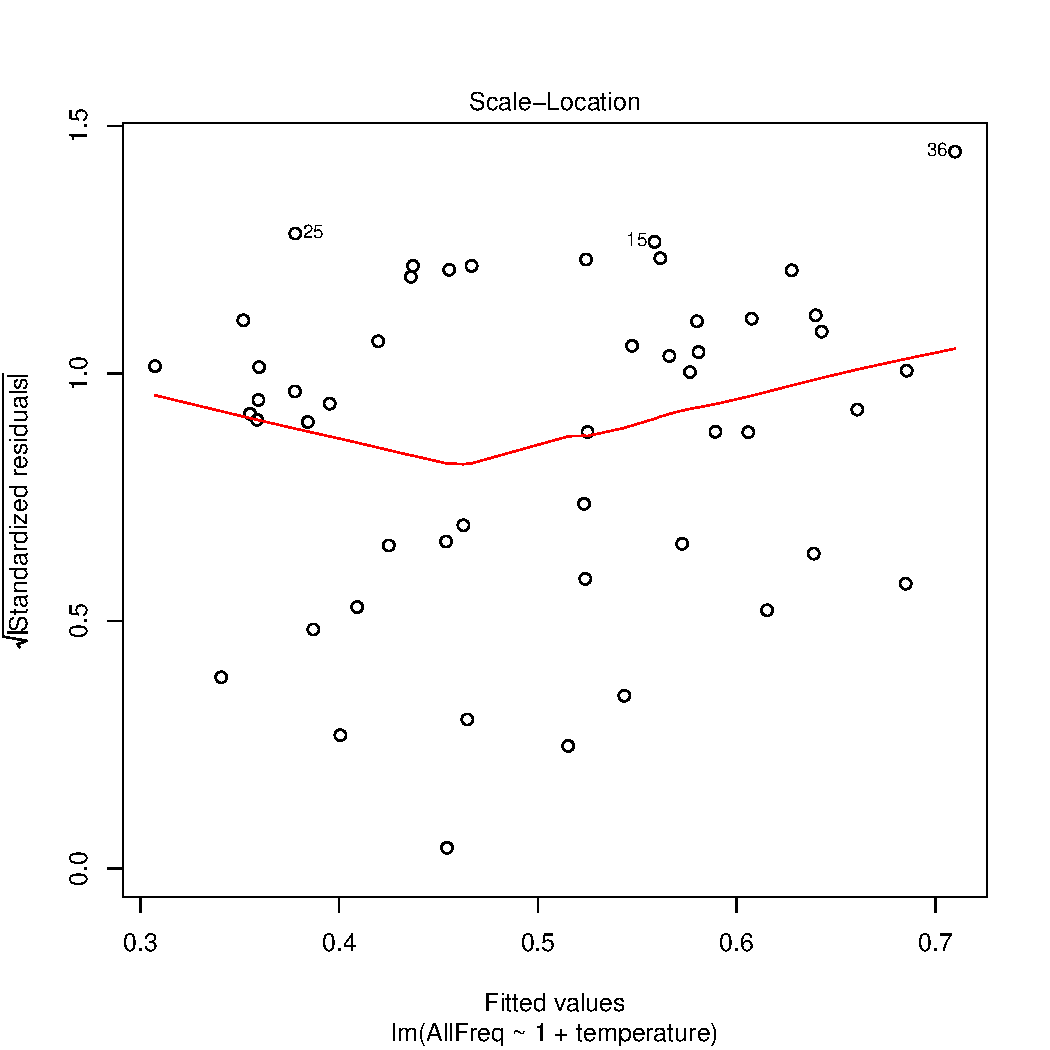
\includegraphics[width=\maxwidth]{figure/unnamed-chunk-12-3} 

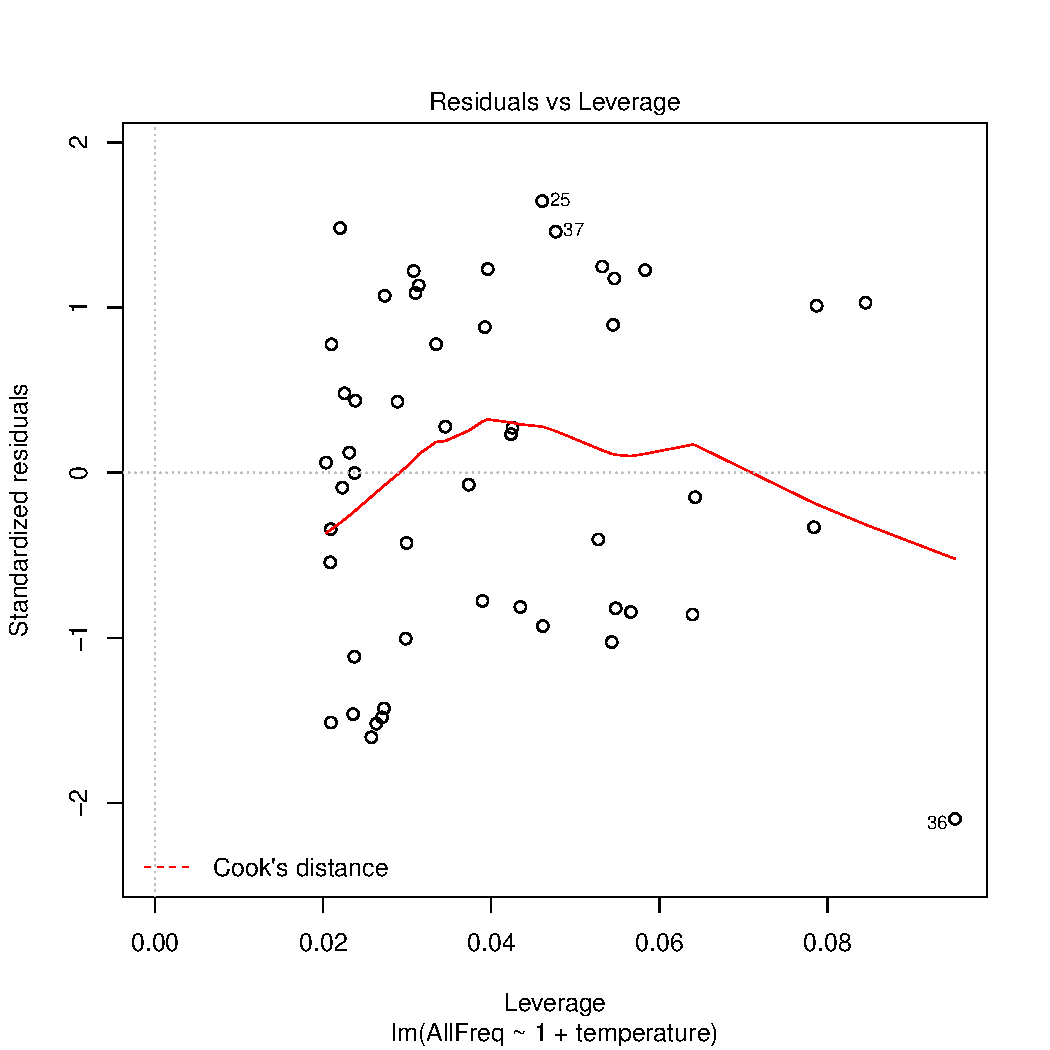
\includegraphics[width=\maxwidth]{figure/unnamed-chunk-12-4} 

\end{knitrout}

The residual distribution is not nice. Maybe we can try a logit transform:

\begin{knitrout}
\definecolor{shadecolor}{rgb}{0.969, 0.969, 0.969}\color{fgcolor}\begin{kframe}
\begin{alltt}
\hlstd{genot}\hlopt{$}\hlstd{logitFreq} \hlkwb{<-} \hlkwd{log}\hlstd{(genot}\hlopt{$}\hlstd{AllFreq}\hlopt{/}\hlstd{(}\hlnum{1}\hlopt{-}\hlstd{genot}\hlopt{$}\hlstd{AllFreq))}
\hlstd{lm1} \hlkwb{<-} \hlkwd{lm}\hlstd{(logitFreq} \hlopt{~} \hlnum{1} \hlopt{+} \hlstd{temperature,} \hlkwc{data}\hlstd{=genot)}
\hlkwd{summary}\hlstd{(lm1)}
\end{alltt}
\begin{verbatim}
## 
## Call:
## lm(formula = logitFreq ~ 1 + temperature, data = genot)
## 
## Residuals:
##     Min      1Q  Median      3Q     Max 
## -1.0704 -0.4455  0.0138  0.5207  0.8437 
## 
## Coefficients:
##             Estimate Std. Error t value Pr(>|t|)    
## (Intercept)  -20.597      3.324    -6.2  1.3e-07 ***
## temperature    1.988      0.321     6.2  1.2e-07 ***
## ---
## Signif. codes:  0 '***' 0.001 '**' 0.01 '*' 0.05 '.' 0.1 ' ' 1
## 
## Residual standard error: 0.538 on 48 degrees of freedom
## Multiple R-squared:  0.445,	Adjusted R-squared:  0.433 
## F-statistic: 38.4 on 1 and 48 DF,  p-value: 1.24e-07
\end{verbatim}
\begin{alltt}
\hlkwd{plot}\hlstd{(lm1)}
\end{alltt}
\end{kframe}
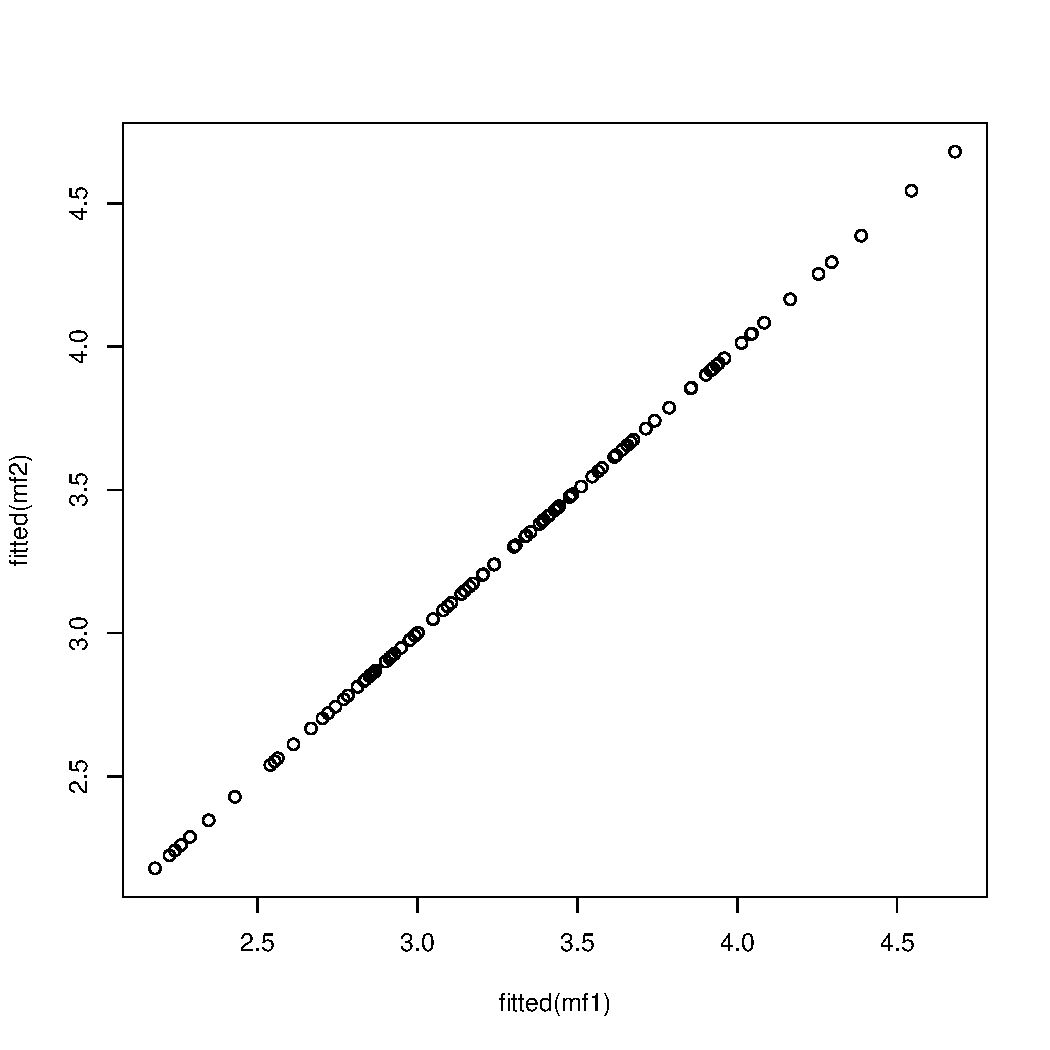
\includegraphics[width=\maxwidth]{figure/unnamed-chunk-13-1} 

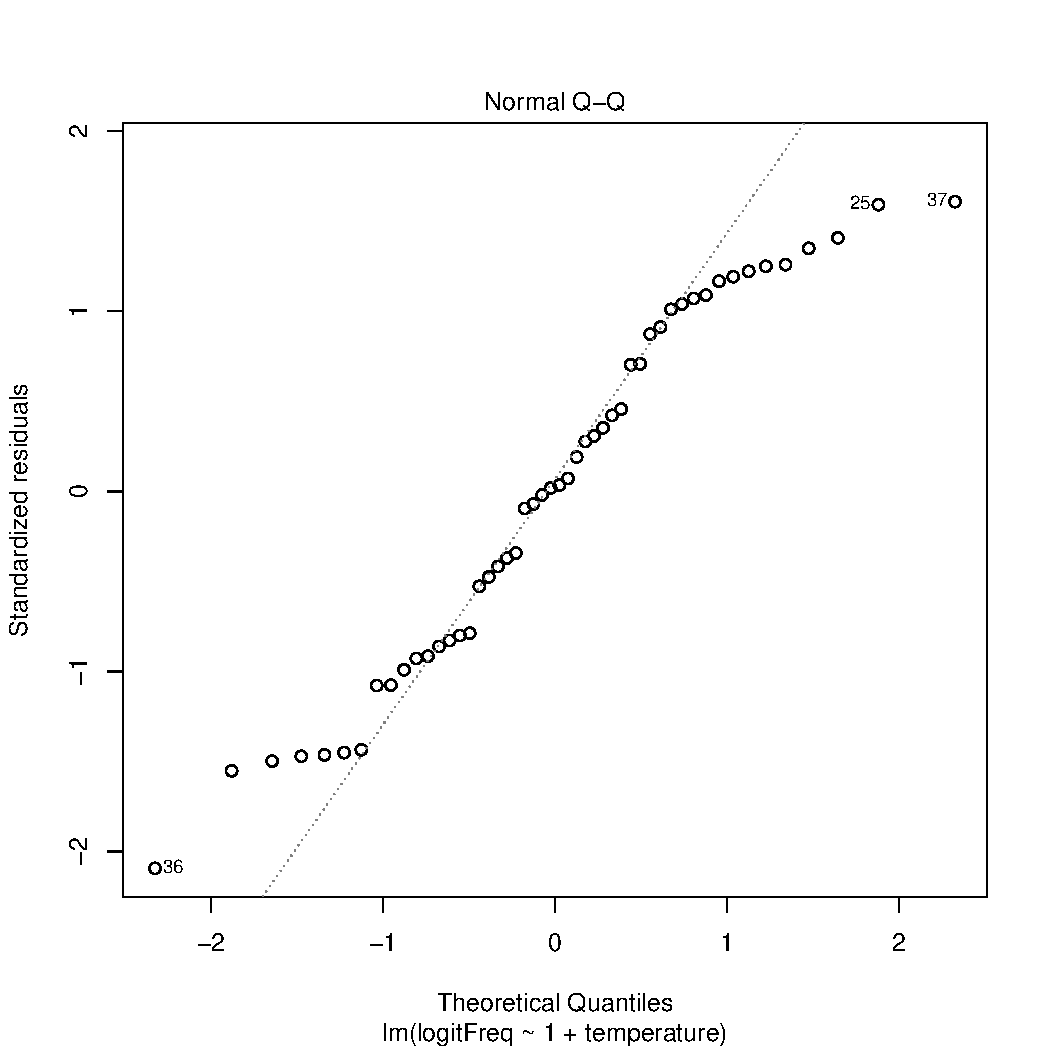
\includegraphics[width=\maxwidth]{figure/unnamed-chunk-13-2} 

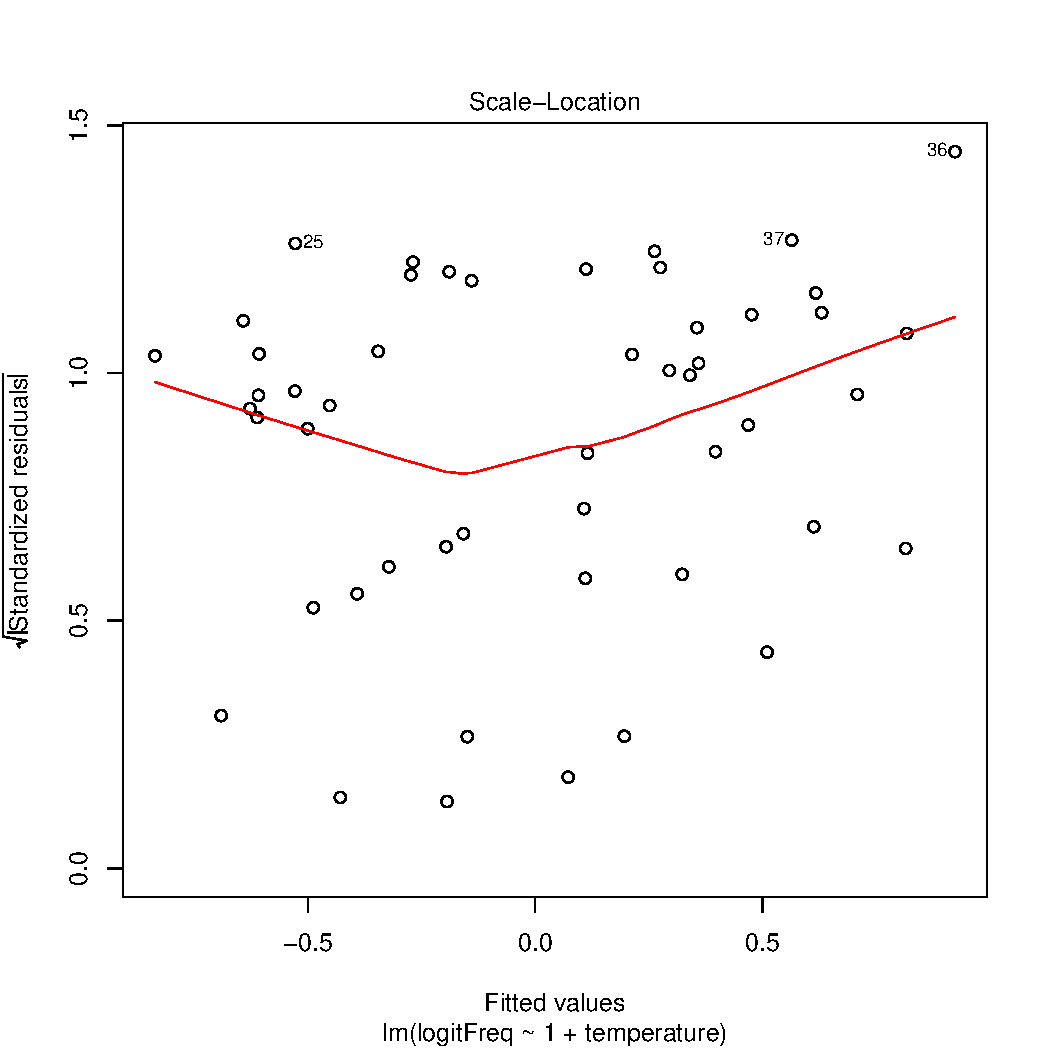
\includegraphics[width=\maxwidth]{figure/unnamed-chunk-13-3} 

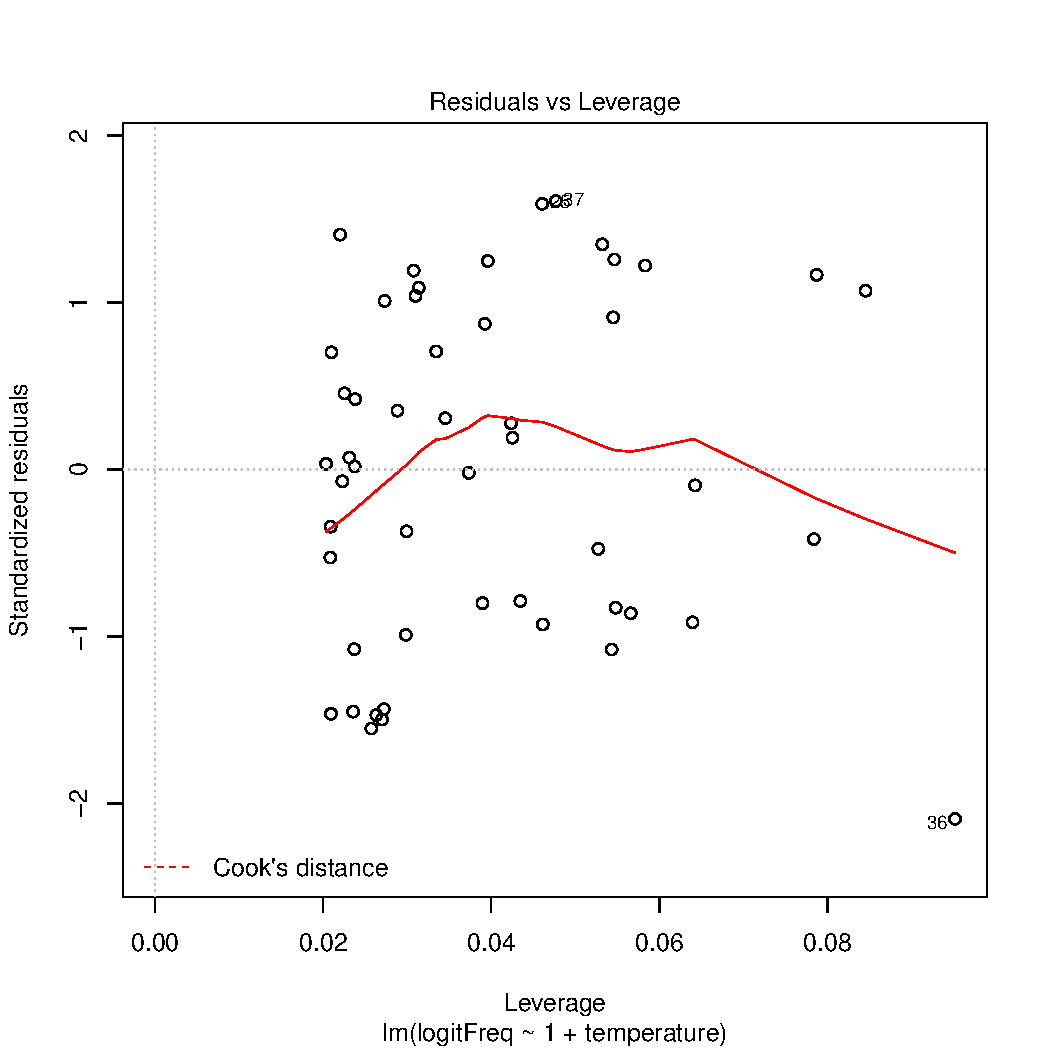
\includegraphics[width=\maxwidth]{figure/unnamed-chunk-13-4} 

\end{knitrout}
Still not great, but that is not the worst. The dataset contains geographic coordinates... what if genetic differences just reflect geographic isolation, which happens to correlate with temperature...

\begin{knitrout}
\definecolor{shadecolor}{rgb}{0.969, 0.969, 0.969}\color{fgcolor}\begin{kframe}
\begin{alltt}
\hlstd{lm2} \hlkwb{<-} \hlkwd{lm}\hlstd{(logitFreq} \hlopt{~} \hlnum{1} \hlopt{+} \hlstd{temperature} \hlopt{+} \hlstd{xcoor} \hlopt{+} \hlstd{ycoor,} \hlkwc{data}\hlstd{=genot)}
\hlkwd{summary}\hlstd{(lm2)}
\end{alltt}
\begin{verbatim}
## 
## Call:
## lm(formula = logitFreq ~ 1 + temperature + xcoor + ycoor, data = genot)
## 
## Residuals:
##      Min       1Q   Median       3Q      Max 
## -0.22574 -0.07769 -0.00512  0.08248  0.26215 
## 
## Coefficients:
##              Estimate Std. Error t value Pr(>|t|)    
## (Intercept)  4.201941   3.668357    1.15     0.26    
## temperature -0.231482   0.283559   -0.82     0.42    
## xcoor        0.022739   0.000727   31.29  < 2e-16 ***
## ycoor        0.113739   0.014112    8.06  2.4e-10 ***
## ---
## Signif. codes:  0 '***' 0.001 '**' 0.01 '*' 0.05 '.' 0.1 ' ' 1
## 
## Residual standard error: 0.113 on 46 degrees of freedom
## Multiple R-squared:  0.976,	Adjusted R-squared:  0.975 
## F-statistic:  637 on 3 and 46 DF,  p-value: <2e-16
\end{verbatim}
\begin{alltt}
\hlkwd{plot}\hlstd{(lm2)}
\end{alltt}
\end{kframe}
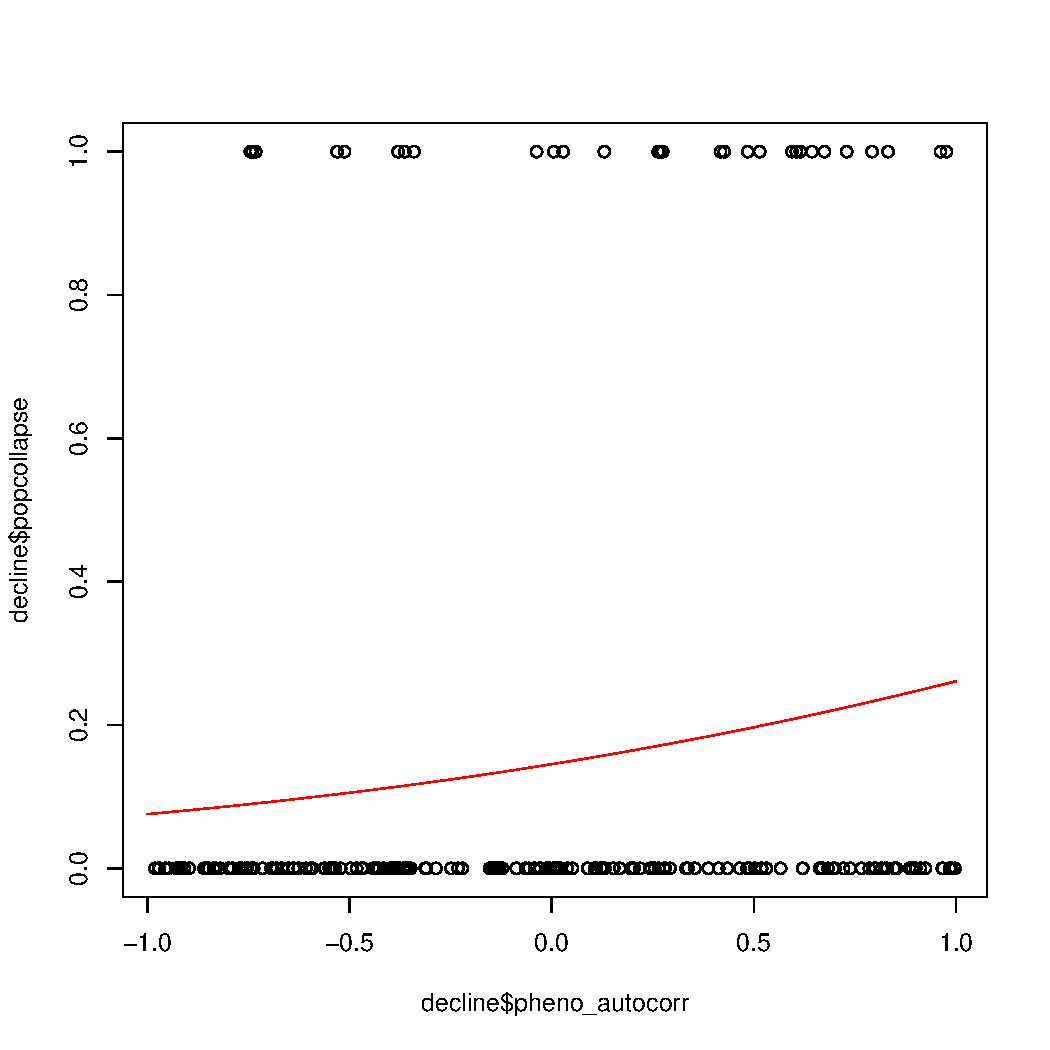
\includegraphics[width=\maxwidth]{figure/unnamed-chunk-14-1} 

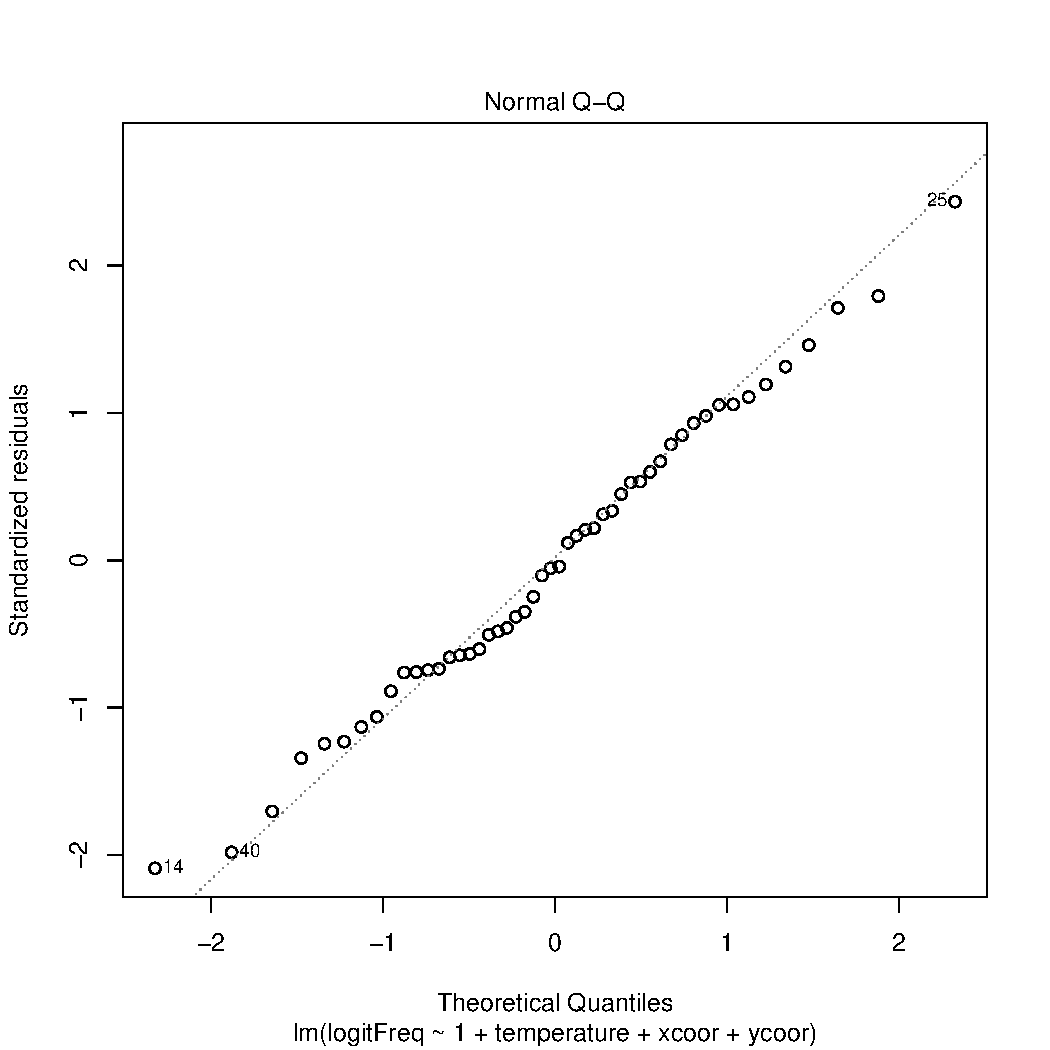
\includegraphics[width=\maxwidth]{figure/unnamed-chunk-14-2} 

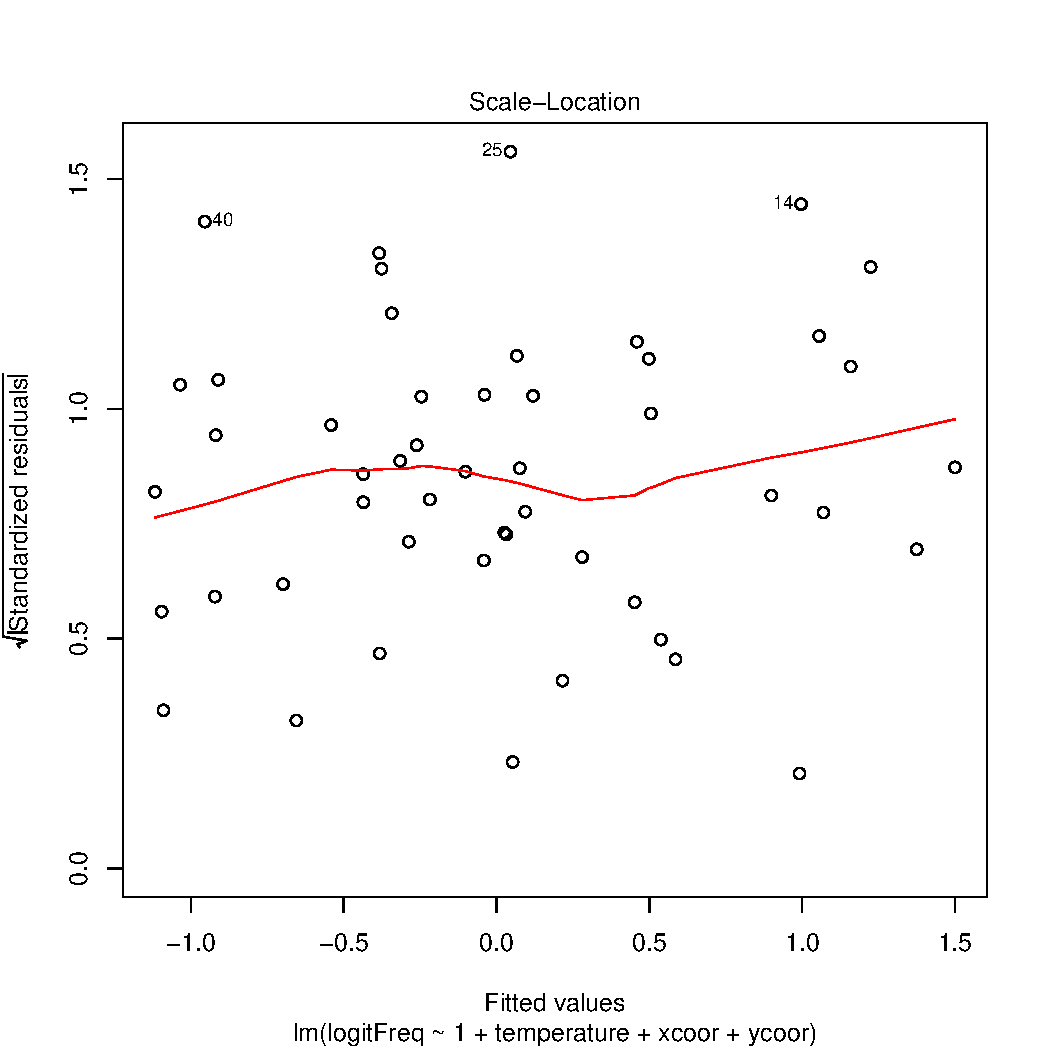
\includegraphics[width=\maxwidth]{figure/unnamed-chunk-14-3} 

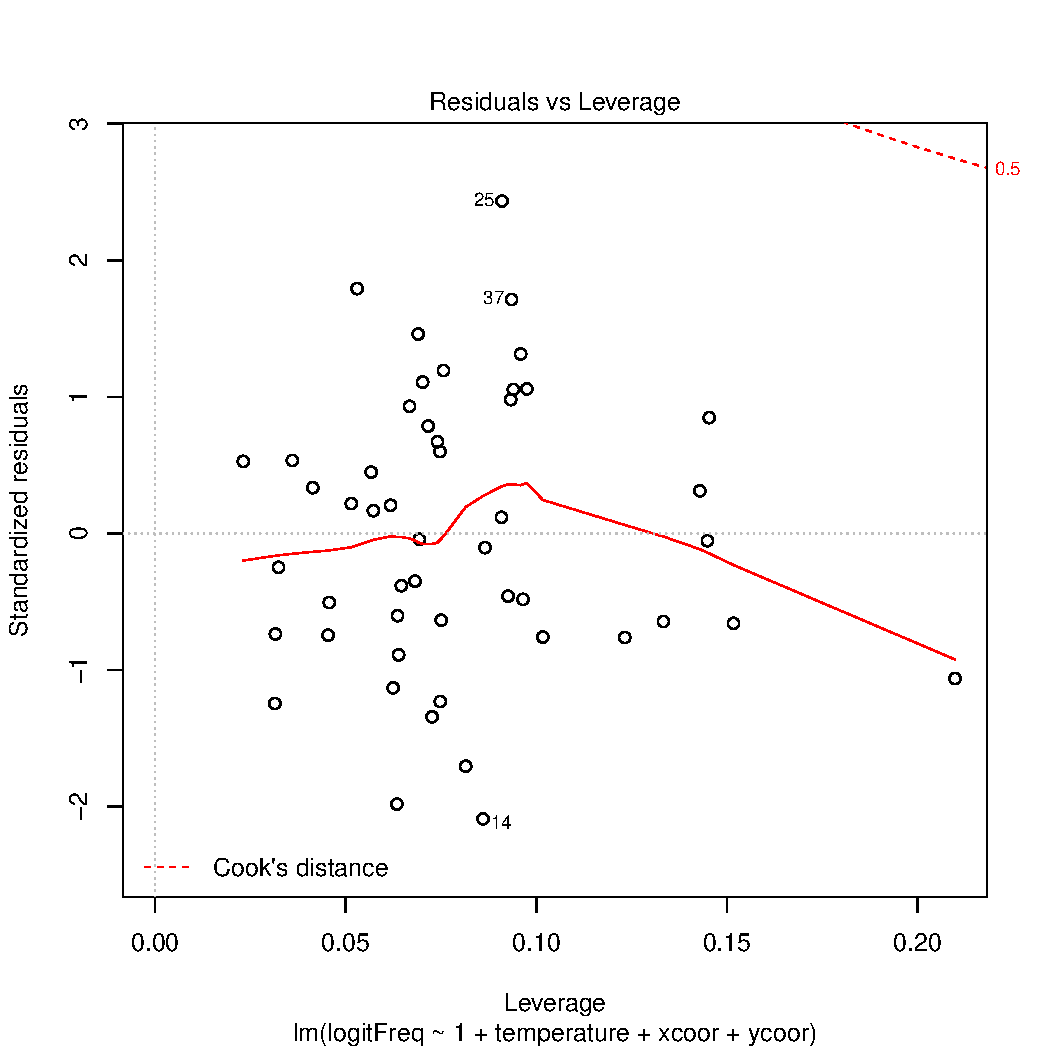
\includegraphics[width=\maxwidth]{figure/unnamed-chunk-14-4} 

\end{knitrout}
Indeed, the effect of temperature disappears once we correct for geography, and also, the residuals now look Normal!
The deeper problem here was non-independence of observations, with non-normality of residuals being more of a decoy...
\end{Answer}

\section{DIY for complex issues}
Knowing how to relax assumptions is a huge topic, pretty much synonymous to knowing how to do statistical modelling. 
We cannot cover all aspects in 2 hours, but we can train to understand what you may want, and learn the name of a few models, so that you can look them up later. So, without worrying about software and code, let's try and imagine what the models would look like (verbally or in equations).

\begin{Exercise}[difficulty=2, title={Measurement error}]
  You have measured body mass in small wild animals, in the field, on windy days. You are trying to quantify how much variation in mass explains survival to the next year. You model survival probability as $p_i \sim logit(\mu + M_i\beta )$ (and $Survial_i \sim Bernouilli(p_i)$), but you know $M$ are not the true masses, but only measurements with a lot or error... that violates a fundamental assumtion of your model. How to write a model that relaxes that assumption? (What new assumptions would you need then?)
\end{Exercise}
\begin{Answer}
$Survial_i \sim Bernouilli(p_i)$; the survival of individual $i$ is a "toss of a coin" with probability of success $p_i$.\\
$p_i \sim logit(\mu + m_i\beta )$; that probability is a linear function (on a logit scale) of a population intercept and the effect of mass on survival multiplied by the individual true mass ($m_i$).\\
$M_{it} \sim Normal(m_i,V_{ME})$; We cannot measure the true mass, but our measurements ($M$) of individual $i$ at different times $t$ follow a normal distribution of mean $m_i$ and variance $V_{ME}$; the variance is assumed to be the same for all individuals and all times.\\

The class of model you want is simply called "Measurement error models". 
\end{Answer}

\begin{Exercise}[difficulty=1, title={Non-linear model}]
You study the effect of temperature on population growth rate in a species of yeast. You start from single cells in bottles and grow populations at 10 different temperatures (3 bottles per temperature) and measure population size at five different times. You know from litterature that population size ($P$) can often be modelled as $P(t) = \frac{K}{1+A\exp(-rt)}$ where $K$ is the carrying capacity, $A$ is a constant we do not care about, $t$ is time, and $r$ is the growth rate.
At first you try to fit the equation above for every bottle, extract the estimate of $r$, and then correlate $r$ with temperature, but you quickly realize this is not ideal, because the estimate of $r$ and all other parameters are very imprecise (you have only 5 points per bottle, and population count data are noisy!) and the error in the estimates of $r$ are not accounted for.

How would you write a model to estimate the effect of temperature on population growth? What assumptions will need?
\end{Exercise}
\begin{Answer}
Possible answer (I do not know enough about micro-biology to be sure it is reasonable!):\\
$P(t) = \frac{K}{1+A\exp(-r_i t)}$, where $r_i$ is the growth rate in a given bottle $i$\\
Optionally, you could consider that your data are $C(t) \sim Normal(P(t), V_m)$, because the count you make may not be an exact count of $P$.\\
$r_i = \mu + T \beta + \epsilon_i$, with  $\epsilon_i \sim Normal(0,V_e)$; $T$ is temperature, $\beta$ is the effect of temperature, the parameter you are interested about.\\
You will probably make assumptions about the distribution of $\epsilon_i$, that is, the noise around growth rate; here we have assumed that $K$ the carrying capacity was a constant, but that does not need to be; we could also fit it as a function of temperature.


This kind of models can bet fitted in the package nlme, or in various bayesian packages. 

\end{Answer}

\begin{Exercise}[difficulty=2, title={When something is missing}]
You study diet in a population of sea elephants on their colony by looking at the isotopic composition of Nitrogen in their blood (different preys are differently enriched in some isotops, so you can tell whether an animal rather eats a lot of invertebrates or a lot of fish).
You suspect animals migrate to two different areas which are known to differ in food resources (one is fish-rich, the other krill-rich), but have no way to observe them there and there are no data on who goes where. You fitted a linear model of concentration in nitrogen-15 with age and sex as covariates. You obtained this distribution for your residuals:

\begin{knitrout}
\definecolor{shadecolor}{rgb}{0.969, 0.969, 0.969}\color{fgcolor}
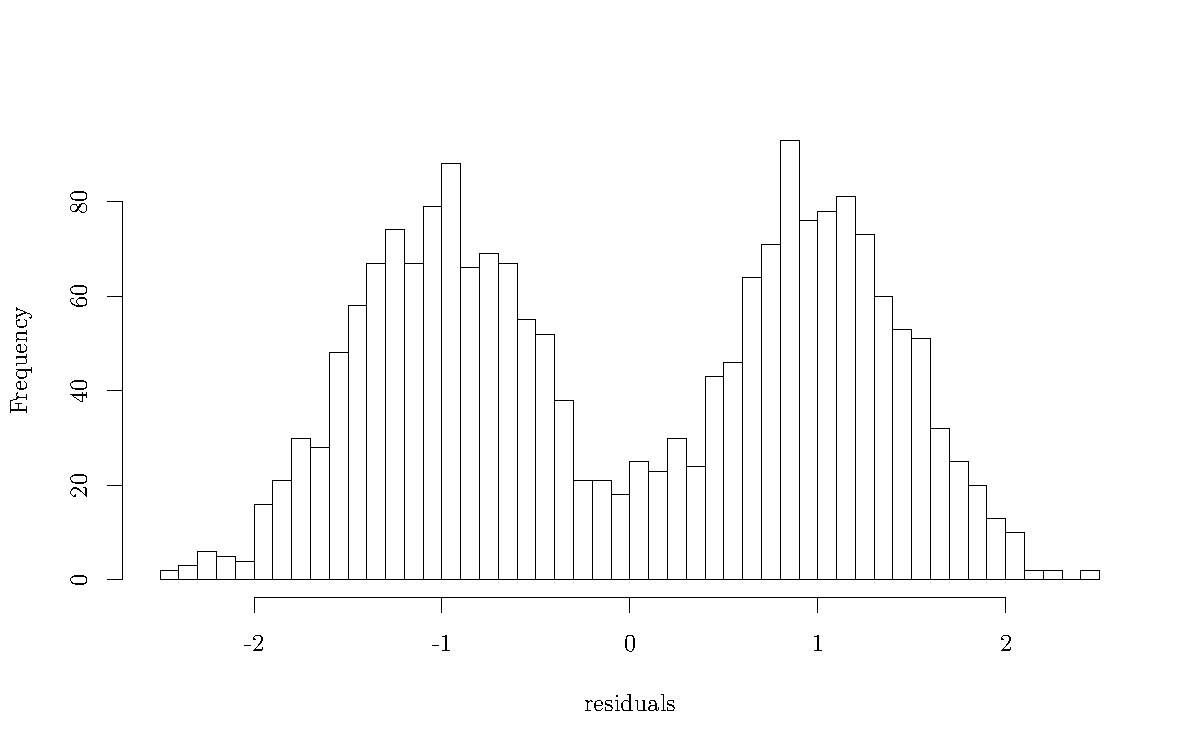
\includegraphics[width=1\textwidth]{figure/unnamed-chunk-15-1} 

\end{knitrout}
What model could you fit to get better residuals, and learn something new? What new assumptions do you need?
\end{Exercise}
\begin{Answer}
These two peaks could correspond to the two migration zones, and we could classify animals based on that.
$N_i = \mu + sex_i\beta_s + age_i\beta_a + m_i + \epsilon$, $ \epsilon \sim Normal(0,V_e)$\\
$m_i \sim Bernouilli(p_i)$, where $p_i$ is the probability that individual $i$ migrated to zone 1.\\

If you have other covariates, like mass, social status... you could try and see if they predict migration!
For instance:
$p_i = logit(intercept + mass * \beta_{mass})$

The model you are after is called a "mixture model". There are relatively easy to fit in bayesian packages like Rjags or RStan.
\end{Answer}

\begin{Exercise}[difficulty=2, title={Markovian process}]
What if the current state of your response variable depends heavily on the previous state. For instance, you study kangaroo movements and have GPS locations every 2 minutes. You try to model habitat selection, but realize residuals are far from independent in your model... How to relax assumptions, what new assumptions would you make?
\end{Exercise}
\begin{Answer}
We may use a model of spatial or time autocorrelation. We may assume that the current location is constrained by the previous location (which assumes that the second time step in the past does not directly matters; which could be wrong). We may also assume that individuals move independently of each others, which could be relaxed using groups as random effects.
\end{Answer}

\end{document}
